\documentclass[a4paper, 11pt]{book}
\usepackage[english]{babel}
\usepackage{amsmath, amssymb}
\usepackage{enumitem}
\usepackage{makeidx}
\makeindex

\newcommand{\version}{Version: October 2024}


% verbatim environment, and fvextra to allow line breaks.
\usepackage{fancyvrb}
\usepackage{fvextra}

\usepackage{natbib}
\bibliographystyle{plainnat}

% typeset inline code
\newcommand{\code}[1]{\texttt{#1}}
% define links
\usepackage[hidelinks]{hyperref}
\newcommand{\hlink}[2]{{\href{#1}{#2}}\footnote{\href{#1}{\code{#1}}}}

\newcommand{\yay}{\textsf{True}}
\newcommand{\nay}{\textsf{False}}

\newcommand{\str}[1]{\texttt{"#1"}}

\newtheorem{definition}{Definition}

\usepackage{pgf}
\usepackage{tikz}
\usetikzlibrary{arrows,automata}

\setcounter{tocdepth}{1}

% 
\usepackage{xcolor}
\usepackage{framed}
\definecolor{shadecolor}{rgb}{0.95,0.95,0.95}

\usepackage{appendix}

% Use a sans-serif font by default
\renewcommand{\familydefault}{\sfdefault}


% shaded box for important terms
\newenvironment{terminology}[1]{
\begin{shaded*}
\textbf{#1\index{#1}.}\\
}
{
\end{shaded*}
}

% No paragraph indentation, skip 2ex instead
\setlength{\parindent}{0pt}
\setlength{\parskip}{2ex}

\title{Topics in data management}
\author{Mark van der Loo}
\date{
\begin{center}

\includegraphics[height=6cm]{fig/bart_simpson_excel_is_not_a_database.jpg}
\end{center}
\version{}\\
\begin{picture}(0,0)
\put(80,500){
\includegraphics[height=2cm]{logo/cbs}\textrm{ }%

\includegraphics[height=2cm]{logo/ul}\textrm{ }%

\includegraphics[height=2cm]{logo/uu}\textrm{ }%

\includegraphics[height=2cm]{logo/emos}}
\end{picture}
}


\begin{document}
\maketitle

\thispagestyle{empty}
\null
\vfill{}
\begin{description}[noitemsep]
\item \version{}
\item This work was created while the author worked at Statistics Netherlands.
      The syllabus was used as a part of the EMOS course on data management
      from 2021 to 2025.
\item To the author's best knowledge, the cover picture was published first
      by Stuart McMillan in the context of the UK government misreporting
      the number of SARS-COVID-19 cases becase of faulty data management using Excel.
      \href{https://twitter.com/mcmillanstu/status/1313520477919498246}{https://twitter.com/mcmillanstu/status/1313520477919498246} 

\item Typeset with \LaTeX{}, \today.
\end{description}




\frontmatter

\section*{Preface}

These notes are based on several versions of a twelve-hour course that was
taught as part of the European Master's of Official Statistics track (EMOS). The
course was given by the author for students of the University of Utrecht (since
2016) and Leiden University (since 2019). The Master's track is followed by a
broad class of studens, but many of them have a bachelor's degree in one of the
social sciences,followed by a research master's with an emphasis on statistics 
and quantitative research. 

The topics have changed a few times during the four years this course was given.
They now cover a range of areas including data validation, the statistical
value chain, data structures, relational data management and more. Although each
topic could only be touched upon given the short time available for the course,
it was always attempted to treat both theoretical and practical aspects. 


\section*{Reading guide}

Important terminology is presented in a frame for easy lookup.
\begin{shaded*}
\textbf{Terminology}\\
Important terms are presented here like this.
\end{shaded*}

Every Chapter has exercises. When there are answers, there is a link to the page
number where you can find the answers below the exercises. You can click on the
link in the section heading of the answers to jump back to the exercises.





\section*{Acknowledgments}


Part of this work was written during a visiting professorship at Universidade
Federal de Pelotas (Br) in 2019, where I taught a four day course on data
management for scientists. I like to thank professors Maximiliano (Max) Cenci,
Tatiana Pereira Cenci and Marcos Britto Correa for their kind hospitality and
pleasant collaboration. The visit was funded by CAPES 
Grant Agreement No 88887.368241/2019-00.

I am greatly indebted to Ronald Ossendrijver for carefully reviewing the
manuscript.  Any errors are of course on account of the author.


\hfill{} Mark van der Loo, October 2020



\newpage
\tableofcontents{}

\mainmatter


\chapter{The faces of data}
\label{sect:faces}
The main purpose of this chapter is to raise awareness of the different ways
data are used, and how and why data should be structured for a specific purpose.
The reader is also acquainted with a few common terms related to data
management.

%%%%%%%%%%%%%%%%%%%%%%%%%%%%%%%%%%%%%%%%%%%%%%%%%%%%%%%%%%%%%%%%%%%%%%%%%%%%%%%
\section{Introduction}
\label{sect:faces:introduction}
Data are created and used for many different purposes, and it should therefore
not be surprising that the same data occurs in different guises that are
geared for a specific type of use.  One of the most common mistakes made in
data analyses or data management is to take data that is structured for one
purpose, say presentation, and try and use it in that form for another purpose like
statistical analyses. The purpose of this chapter is to give an overview
of the main types of uses of data, the way data is typically structured for
each purpose, and to compare their relative advantages and disadvantages.




The main uses of data distinguished here are storage, transport, analyses, and
presentation. Each use comes with its own conventions of how to
structure and manipulate data that stem from the different demands that the
different uses imply. For example, for reliable storage, retrieval and updating
of information it is beneficial to store each piece of information exactly
once, while it may be beneficial for interactive data analyses to have multiple
copies of the same data available.  Similarly, when transporting data from one
computer system to another, it is important that data can be `packed' and
`unpacked' quickly with a variety of tools. When presenting data, it is
important that the relevant information can be grasped quickly by users.


Working with data is more comfortable when data is structured especially for a
specific purpose. As a trade-off the other purposes suffer: data formatted for
communicating between web services is hardly fit for human interpretation. One
important aspect of data management is therefore the ability to recognize the
task at hand and transform data into a suitable format. 

As an example, consider a table of (fictional) CO$_2$ emission figures by fuel
source. Pay special attention to how the data are formatted.
\begin{equation}
\begin{tabular}{rl}
\multicolumn{2}{l}{CO$_2$ emission (kiloton per annum)}\\
\hline
\textbf{fuel}    & \textbf{emission}\\
\hline
\multicolumn{1}{l}{Petrol}      & 215 \\
-- of which bio                  & \phantom{0}75  \\
\multicolumn{1}{l}{Diesel}     & 456 \\
-- of which bio                  & \phantom{0}89  \\ 
\hline
\end{tabular}
\label{eq:present}
\end{equation}
This type of format is very common. One frequently encounters it for example in
official statistics publications or in financial reports of businesses.
Table~\eqref{eq:present} is optimized so people can quickly eyeball the
contribution of biofuels as a fraction of total emissions for each fuel type.
As a trade-off this table is not very suited for analysis. For example, to
derive the contribution of regular fuels, one needs to subtract the emission
value in the second line from the value in the first line, and do this again
for line three and four. Performing such calculations is much easier, and less
error-prone when the analyst does not have to worry about in what line which
data item is stored exactly.


This situation can be improved by realizing that the first column actually
hides a two-level classification: fuels are split into Petrol and Diesel
while each of those is split into the bio and regular type. Knowing this, the
same information can be represented as follows.
%
\begin{equation}
\begin{tabular}{rrl}
\hline
\textbf{fuel}      & \textbf{type}  & \textbf{emission}\\
\hline
Petrol & regular  & 140 \\
Petrol & bio      & \phantom{0}75\\
Diesel& regular  & 367 \\
Diesel& bio      & \phantom{0}89\\
\hline
\end{tabular}
\label{eq:analyse}
\end{equation}
%
The totals represented in the first table are no longer explicitly represented in
Table~\eqref{eq:analyse}. This is because the totals in Table~\eqref{eq:present}
present the result of an analyses while Table~\eqref{eq:analyse} represents the
basis of an analyses, that is: the raw underlying data. The benefit of the
second representation over the first is that it allows for more general analyses
like computing the total contributions of regular and biofuels.

A good way to think of the difference is that Table \eqref{eq:present} is a
presentation of results, while Table \eqref{eq:analyse} represents a data set
for analyses.  The advantage of the second for over the first is that it allows
general analyses, like computing the total emission contribution of regular
fuels.  Thus, although both tables communicate the same information they differ
in area of application. Unfortunately, the presentation form is very often used
in analyses, especially in spreadsheet software.


Next, have a look at the following format, where the data has been transformed
to a machine-readable string of characters.
%
\begin{equation}
\begin{minipage}{0.9\linewidth}
\begin{Verbatim}[breaklines=true]
[{"fuel":"petrol","type":"regular","emission":140}, {"fuel":"petrol","type":"bio","emission":75}, {"fuel":"diesel","type":"regular","emission":367}, {"fuel":"diesel","type":"bio","emission":89}]
\end{Verbatim}
\end{minipage}%
\label{eq:machine}
\end{equation}
%
Here the little $\hookrightarrow$ indicates that a line break was inserted only
to fit the code on the page. The actual string has no spaces and no line
endings or newlines.  The format presented here is called javascript object
notation (JSON).  The main purpose of this format is to provide a general way
to represent all sorts of data in a standardized way so it can be sent from one
piece of software to another. Now there are many of such formats, but this
particular one is very commonly used for communication between web services and
clients. Clearly, this format is not meant for presentation to people or for
statistical analyses. One advantage of JSON is that it is very generic: data
need not fit in a table to be stored in a JSON string, and in principle any
kind of data can be packed as JSON. Another advantage is that all wide-spread
programming languages have libraries that allow programmers to read, write, and
manipulate JSON data. It is thus a good format to interchange data between
different systems.


Finally, consider the same information but now organized as it would be, 
when stored in a database.
%
\begin{equation}
\begin{tabular}{ll}
\multicolumn{2}{l}{Fuel}\\
\hline
\textbf{id} & \textbf{name}\\
\hline
11 & petrol  \\
12 & diesel \\
\hline
\end{tabular}\textrm{, }\:
%
\begin{tabular}{ll}
\multicolumn{2}{l}{Type}\\
\hline
\textbf{id} & \textbf{name}\\
\hline
1 & regular \\
2 & bio \\
\hline
\end{tabular}\textrm{, }\:
%
\begin{tabular}{llll}
\multicolumn{3}{l}{Emission}\\
\hline
\textbf{id} & \textbf{fuel} & \textbf{type} & \textbf{amount} \\
\hline
120 & 11 &1 &140\\
121 & 11 &2 &\phantom{0}75\\
123 & 12 &1 &367\\
124 & 12 &2 &\phantom{0}89\\
\hline
\end{tabular}
\label{eq:database}
\end{equation}
Now each classification and each concept is given it's own table. There is a
`Fuel' table where each fuel is given a meaningless identifying number, and a
name. The same happened for the subclass `Type'. The table on emission sources
now has a unique id for each emission, and the fuel and type are identified by
the id's in their respective table. The reason data is stored in such a format
in database systems is that they are optimized for consistency. For example, if
one needs to replace the fuel name `petrol' with `gasoline', then the formats
presented in \eqref{eq:present}, \eqref{eq:analyse}, and \eqref{eq:machine}
require multiple changes in multiple places, which is both inefficient and
error-prone.  The database format ensures that in case of an update, only a
single item needs to be touched and everything else is updated immediately.
This benefit of easy and consistent updates comes with a cost: the data in the
Emission table is not understandable unless one knows the other tables as well.
We shall go into more detail when we discuss relational data in
Chapter~\ref{sect:relational}.

The above examples give some intuition to why it is important to structure data
in a way that is suited for purpose. Below the main types of uses, specific
demands that come with it and typical tools are summarized.

\paragraph{Storage.} When data is formatted for storage, this is typically done
with the four basic operations in mind that are often referred as the CRUD
operations.
\begin{terminology}{CRUD}
Creating, Retrieving, Updating, and Deleting data.
\end{terminology}
To facilitate this, data storage systems must have a way of uniquely
identifying each data item entrusted to them, regardless for example of the
order in which the data is stored.  The database example \eqref{eq:database}
satisfies extra demands such as a form of consistency, but there are other
storage solutions that do not satisfy this consistency but that do support CRUD
operations. Software for data storage is often characterised as either
relational or non-relational. The table set in \eqref{eq:database} is an
example of how data is structured in a relational database. Examples of
non-relational databases include key-value stores, document databases or graph
(network) databases. 

\paragraph{Transport.} When transporting data from one machine to another, it
is important that every value can be packed, send, unpacked and recognized
correctly. Over time many standards have been developed. Important formats
include the JSON format that was mentioned earlier and XML (eXtensible Markup
Language). Both formats are supported by many programming languages and they
can therefore be used by developers to exchange information between systems. 
The formats still leave a lot of choice for how to store data precisely. For 
example, in \eqref{eq:machine}, the order of variables in each record is
fuel--type--emission. Changing this order would still yield a valid JSON
format. For this reason, developers usually fix the way a JSON or XML document
must look like in something called a schema.
%
\begin{terminology}{Schema}
A schema describes the structure of a data format for a
specific type of data, within a chosen standard (e.g. XML, JSON).
\end{terminology}
%
Both \hlink{https://json-schema.org/}{JSON} and
\hlink{https://www.w3schools.com/xml/schema\_intro.asp}{XML} have their own
ways of denoting a schema. Some schemas are fairly simple, such as the JSON
schema defined by the European Statistical System for exchanging information
about
\hlink{https://ec.europa.eu/eurostat/cros/content/validation-report-structure\_en}{data
validation results}. Other schemas are large and elaborate, such as the
\hlink{https://sdmx.org}{SDMX standard}, for standardized exchange of
statistical information between institutions. 


\paragraph{Analysis.} To analyze data interactively, it is important that it is
formatted so that typical operations such as filtering, plotting, and modeling
are made as easy as possible. The most important demands are that a data set
represents a single type of entity and that each data item represents the
properties of one unique entity. Furthermore, there should be no duplicate
entries and all properties should be stored in the correct type (integer,
numeric, nominal, ordinal, text).  
%
\begin{terminology}{Entity type, population, entity, population unit, attribute, variable}
In computer science and specifically in the area of databases, the term \textit{entity
type} refers to a collection of real-world objects or events such as persons, clicks
on a web page, buildings in some city, and so on. In statistics this concept is usually
referred to as a \textit{population}, or target population.

Similarly, in computer science an \textit{entity} is an instance of an entity
type, while in statistics one often refers to a population element as a
\textit{population unit}.

All elements of a population (entities of an entity type) share a set of
properties.  Computer scientists often refer to a property as
\textit{attributes} while statisticians call them \textit{variables} or
\textit{stochastic variables} when probabilistic properties of the data are
important.
\end{terminology}
%
In many, but not all cases (See Section~\ref{sect:faces:types}) this means that
data is represented in a tabular format such as \eqref{eq:analyse} where each
row represents one entity, each column represents one attribute and  each
entity appears only once. A good rule of thumb to decide whether a tabular data
set is fit for analyses is to answer the question: are summary statistics of
the attribute columns meaningful? Compare for instance
Tables~\eqref{eq:present} and~\eqref{eq:analyse}: is it meaningful to compute
the sum of the numeric column? 

\paragraph{Presentation.} The main purpose of data in a presentable format is
to convey a message as clearly and objectively as possible. This means that
presentation is adapted to the expected audience and one may even choose
different presentations for different audiences. Typical tools for data
presentation include spreadsheet software, or business intelligence software
like Tableau. Almost all statistical software packages also offer some kind of
support for data presentation.


In practice, the lines between various uses of data are often blurred by
software tools. Spreadsheet software is optimized for presentation of data but
also offer limited analytical and data management features. Many commercial
databases offer some form of in-database analytical capabilities mixing storage
and analyses while users of spreadsheet software often confuse a spreadsheet
file with a data storage format. Although this blurring can seem convenient it
is almost always better to separate concerns and choose a specialized tool and
data format for the task at hand. The main reason for this is that
reproducibility, maintainability and understandability suffer when a tool is
used for purposes for which it is not designed.  Notorious examples include
complex interlinked sets of spreadsheets where it is very difficult to track
how the results are derived. The lack of systematic testability as well as
their opaqueness renders spreadsheets all but useless for reliable and
reproducible research. They do shine when it comes to presentation, with
features like conditional formatting or interactive pivoting. A second example
of such misuse of a tool is when programming a data analyses in Structured Query
Language (SQL). SQL is optimized for CRUD operations on data bases, but
expressing analytical operations such as computin summary statistics or
model parameters cumbersome when expressed in pure SQL. This then tends to lead
to code that is hard to read and difficult to maintain. So as a general rule,
it is a good idea to choose the data structure and associated tools that are
designed for a specific type of use. 





%%%%%%%%%%%%%%%%%%%%%%%%%%%%%%%%%%%%%%%%%%%%%%%%%%%%%%%%%%%%%%%%%%%%%%%%%%%%%%%
\section{Data types and data manipulation}
\label{sect:faces:types}
We have seen that data can be formatted in different ways for different
purposes.  The structure we use ---a database schema, a JSON string, in principle
says nothing about the \emph{intrinsic} structure of data, which is the
discussion of the following paragraphs.

\paragraph{Relational data.} 
The running example of the previous section is a data set where there is little
intrinsic relation between the different data points. The only intrinsic
structure is the fact that each entity is endowed with a number of attributes.
The way this data is represented has no real meaning: the order of columns and
rows in Table~\ref{eq:analyse} is of no importance. As long as we know which
values belong to which attribute of which entity, the content of the data stays
the same. Any analyses performed on this dataset will be insensitive to
permutations of rows or columns as long as we refer to the columns by their
name rather than position. Data satisfying this requirement is called
`relational data': each relation (row in a table) represents values of
attributes of a single population unit. Typical operations that one performs on
relational data include filtering or sorting rows, or adding or deleting
columns. These operations consume relational data and produce relational data.
The result of certain analyses can also be meaningfully stored in a relational
data set. For example grouped aggregation.

There are many cases where data points represented in a data set do possess
intrinsic interrelations, and this always requires specialized theoretical and
computational tools to analyze. Let us look at some important practical
examples.

\paragraph{Time series.} A time series is a sequence of values (or
value-tuples) that correspond to a sequence of equidistant times or periods.
Examples include monthly GDP estimates, daily closing levels of the stock
market or quarterly estimates of immigration. Many outputs in official
statistics are as time series,  and much effort is spent on constructing them.
Important operations performed on economic time series include inflation
correction, taking account of calendar effects, decomposition into trend and
seasonal effects, decomposition into long-term trend and business cycle
effects, increasing or decreasing the frequency by disaggregation or
aggregation, and more. All these operations have in common that they they both
accept and produce time series. They make explicit use of the fact that data is
organized as a time series and are therefore not invariant under permutation of
the elements of a time series.

\paragraph{Geospatial data.} This data type is used to visualise and analyse
phenomena where geographical location or geospatial patterns are important.
Some examples from official statistics where geospatial analyses plays a role
include land use, population density, biodiversity, and environmental
accounting. In geospatial data, each value is related to a point, line, or
region (a polygon) that is represented in a certain co-ordinate system.
Typical operations include co-ordinate transformations, geospatial smoothing,
and merging or splitting of regions. Again, permuting the values with respect
to their geospatial features (point, line, region) would make such operations
useless. Also observe that again, the `typical operations' mentioned here both
consume and produce geospatial data.


\paragraph{Network data.} A network consists of nodes, connected by links.
Nodes represent entities while links represent connections between them.  For
example a client--server relationship between companies, a family link between
persons, or a shared employer between persons.  At the time of writing,
official statisticians are just beginning to explore the uses of network data,
but it is likely that a more `systemic' approach to describing the economy and
society based on network science will play a role in the future of official
statistics. For networks, the structure \emph{is} the data. In network analyses
one is interested in summarizing or using network structure as a means to gain
insight in the phenomenon described by it. Typical operations on networks
include subnetwork selection or CRUD operations like adding or deleting nodes
or links. Again (and notice this is becoming a theme now), these operations
consume and produce networks.


\paragraph{Other.} There are many more data types that are useful but not
naturally represented in relational format. Examples include images, videos, or
event logs. All these data types come with their own `natural' transformations.

By now, attentive readers have probably detected a recurring theme across
these examples. Each data type comes with a set of `natural' operations that
leave the data type intact. This phenomenon is so important that mathematicians
and computer scientist have a name for it.
\begin{terminology}{Algebraic closure} Given
a data type $T$, and an operation that manipulates data of that type.  We say
that $T$ is \emph{algebraicly closed} under this operation when the result of
the operation is again of the same type $T$.
\end{terminology}

In practice, things are easier when you work in an algebraically closed system
of operations. For example. Given a relational data set, we can develop a
script where we first filter, then sort, and then merge the data set with
another data set. These operations are easy to perform in sequence because the
output of one operation can serve as input to the next. If we discover a bug
and find out we need to merge before filtering, the only thing we need to do is
swap the two operations. Indeed, working within an algebraically closed system
feels so natural that one can focus on \emph{what} of the data manipulation,
rather than at the \emph{how}.

There are other advantages that are facilitated by algebraic closure. For
example, most modern database systems are capable of re-ordering instructions
to increase speed of execution. For example it is faster to first filter
records and then sort them then the other way around (because there is less to
sort that way). Algebraic systems generally come with a set of re-ordering
rules that can be taken advantage of by software that executes it. Important
examples of algebraic systems are the various query languages that implement
CRUD operations for different data types. Examples include Structured Query
Language (SQL) for relational data, Cypher for network data and Spatial SQL for
geographic data.


The main takeaway of this section is that it is useful to distinguish between
\emph{data transformations} where data is manipulated but the type does not
change, and \emph{type transformations} where data manipulation yields data of
a new type. Third, we saw in \S\ref{sect:faces:introduction} there are format
transformations that change the technical layout of data. 

A typical step in a statistical production system starts with reading data from
a file or database. This is a format transformation, possibly followed by a
type transformation. For example when a JSON string is read into a relational
format. Next, depending on the task several type-conserving transformations
and/or type-transforming data manipulations are carried out after which the
data is again formatted for output.


\section*{Where are we?}
We have seen that data is a representation of information, and that data may be
formatted in several ways depending on its intended use. We have also seen that
data types can be distinguished by looking at their intrinsic structure.
Depending on intrinsic structure, a number of `natural' operations are
associated with data that leave its characteristic structure intact. It is
useful to distinguish between formatting, type-conserving, and type-changing
data transformations.



\newpage{}
\section{Exercises}
\label{sect:exfaces}
\begin{enumerate}
  \item Explain why Table~\eqref{eq:present} is unsuited for storage or transport of data.
  \item Acquaint yourself with storage solutions by reading through the Wikipedia
  entries for \hlink{https://en.wikipedia.org/wiki/Database}{Database} and
  \hlink{https://en.wikipedia.org/wiki/NoSQL}{NoSQL}.
  \item Find out what OLTP and OLAP means.
  \item Explain why or not the following data structures are suitable for analyses.
  \begin{enumerate}
      \item 
          \begin{tabular}{|r|lll|}
          \hline
                    & Alice & Bob & Carol \\
          \hline
          Shoe size & 38    & 43  & 41    \\
          Income    & 3300  & 2800& 4000  \\
          \hline
          \end{tabular}
      \item 
          \begin{tabular}{|r|llll|}
          \hline
            Income   &   0k -- 20k   &  20k -- 40k  &  40k -- 80k   & 80K+ \\
          \hline 
           Amsterdam & 20\%          &   40\%       &   35\%        & 5\%  \\
           Rotterdam & 30\%          &   30\%       &   38\%        & 2\%  \\
           Den Haag  & 25\%          &   35\%       &   30\%        &10\%  \\
          \hline
          \end{tabular}

      \item
          \begin{tabular}{|r|ll|}
          \hline
           Name & Age  &has job \\
          \hline
           Dave & 36   &No      \\
           Eve  & 5    &Yes     \\
          \hline
          \end{tabular}
      \item
\begin{tabular}{|r|ll|}
\hline
 Sector      & costs  &profit \\
\hline
 Retailers   & 50     &10     \\
 Wholesalers & 20     & 5     \\
 Total       & 70     &15     \\
\hline
\end{tabular}


  \end{enumerate}
\item Name three operations on image data that leave the data type intact.
\item Explain why each of the following statements is true or false.
\begin{enumerate}
  \item The natural numbers $\mathbb{N}=\{1,2,\ldots\}$ are closed under multiplication.
  \item The rational number s $\mathbb{Q}$ are closed under addition.
  \item The real numbers $\mathbb{R}$ are closed under division.
  \item We denote with $\Sigma^*$ the set of all finite strings that can be
    created with an alphabet $\Sigma$. For example if $\Sigma=\{a,b,\ldots,z\}$
    then $\Sigma^*$ is the set of all finite concatenations of letters from the
    Latin alphabet, plus the empty string (the string without characters).
    Statement: $\Sigma^*$ is closed under concatenation of strings (pasting one
    string behind the other).
 \item The function $\textrm{zero}$ returns $0$ for each value it is given. For
       Example $\textrm{zero}(\pi)=0$. Statement: the integers $\mathbb{Z}=\{\ldots, -2, -1, 0, 1, 2,\ldots\}$ are closed under $\textrm{zero}$.
 \item The natural numbers are closed under $\textrm{zero}$.
 \item (Bonus question) The function $a_n$ adds the number $1$, $n$ times to
    its input.  For example $a_3(2)=2+1+1+1=5$. Statement: the natural numbers are
    closed under $a_\infty$.
\end{enumerate}
\end{enumerate}

\hfill{}Check your answers on page~\pageref{sect:ansfaces}.



\chapter{The statistical value chain}
\label{sect:valuechain}
In this Chapter we look at some general principles that help to organize data
processing, going from raw data to statistical output\footnote{Partly based on
\citet[Chapter 1]{loo2018statistical}}.


\section{Statistical value chain}
A national statistical institute (NSI) can in many ways be seen as a data
factory.  Indeed, both nationally and internationally official statisticians
refer to their work as `production', to their data as 'raw data' and to their
statistics as 'output'. All terms that are borrowed from phyiscal production
processes. In this sense it is no surprise that the idea of a Statistical Value
Chain has become the preferred way of organizing statistical production in many
statistical offices.
%
\begin{terminology}{Value chain}
The idea of the value chain is based on the process view of organizations, the
idea of seeing a manufacturing (or service) organization as a system, made up
of subsystems each with inputs, transformation
processes and outputs \citep{ifm2013}.
\end{terminology}
%
A value chain, roughly, consists of a sequence of activities that step by step
increase the value of a product. The idea of a statistical value chain has
become a common term in the official statistics community over the last two
decades or so, although a single common definition seems to be
lacking\footnote{One of the earliest references seems to be by
\citet{willeboordse2000statistics}}. Roughly then, a statistical value chain is
constructed by defining a number of meaningful intermediate data products, for
which a chosen set of quality attributes are well-described
\citep{renssen2008standardisation}.  There are many ways to go about this, but
the picture shown in Figure~\ref{fig:valuechain} has proven to be a fairly
generic and useful picture to organize thoughts around a statistical production
process. 
%
\begin{figure}
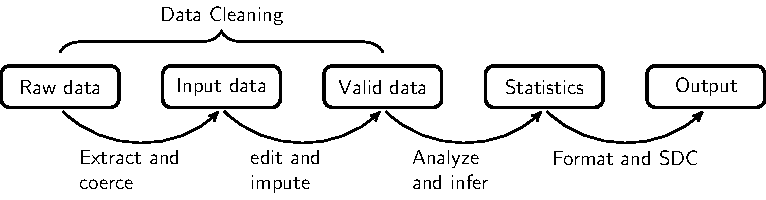
\includegraphics[width=\textwidth]{fig/valuechain.pdf}
\caption{Part of a statistical value chain, showing five different levels of 
statistical value going from raw data to statistical product.}
\label{fig:valuechain}
\end{figure}
A nice trait of the schema in Figure~\ref{fig:valuechain} is that it naturally
introduces activities that are typically categorized as `data cleaning' into
the statistical production process. From the left we start with raw data.  This
must be worked up to satisfy (enough) technical standards so it can serve as input
for consistency checks, data correction and imputation procedures.  Once this
has been achieved, the data may be considered valid (enough) for the production
of statistical parameters. These must then still be formatted to be ready for
deployment as output. 



More generally, a statistical production process is designed by viewing
input, output and a number of intermediate states as statisitical products.
\begin{terminology}{Statistical product}
A state of data that is guaranteed to satisfy a predifined set of quality
demands. 
\end{terminology}
Thus each state, represented by a rectangle in Figure~\ref{fig:valuechain} is
fixed by specifying precisely when a data set is allowed to be called `raw', or
`valid' and so on. Physically, each state may be represented by a table in a
data base, a set of files, or any other way data can be represented. A
description should be accurate enough to understand the contents of a data set
as well as the limits of its usability. To describe usability, the five quality
aspects defined in the Eurpean Quality Assurance Framework (QAF): relevance,
accuracy, timeliness, accessibility and comparability serve as a guide of
things to describe. For example, a good description of the file format falls
under accessibility while an accurate description of logical restrictions that
the data satisfy (like `Age is nonnegative') falls under 'accuracy and
reliability'.


\begin{terminology}{The five quality aspects of data}
  In the European Quality Assurance Framework, the following five quality 
  dimensions are defined.
  \begin{itemize}
    \item\textbf{Relevance.} The degree to which the statistical product meets
    user needs in both coverage
    and content.
    \item\textbf{Accuracy \& Reliability.} Accuracy is the proximity between an estimate
    and the unknown true value. Reliability is the closeness of early estimates to
    subsequent estimated values.
    \item\textbf{Timeliness and Punctuality.} Timeliness refers to the time gap between
    publication and the reference period. Punctuality refers to the gap between
    planned and actual publication dates.
    \item\textbf{Accessibility and Clarity.} Accessibility is the ease with which users are
    able to access the data, also reflecting the format in which the data are
    available and the availability of supporting information. Clarity refers to the
    quality and sufficiency of the metadata, illustrations and accompanying advice.
    \item\textbf{Comparability and Coherence.} Comparability is the degree to which data
    can be compared over time and domain. Coherence is the degree to which data
    that are derived from different sources or methods, but refer to the same
    topic, are similar.
  \end{itemize}
\end{terminology}

Having solid descriptions of each state are an important step of making data
usable for other production processes or incidental analyses.  It makes
different statistical production chains composable by using the output of one
chain as input for another.  The definition of statistical products allows one
to systematically disentangle a complex set of activities going from input to
output into manageable chunks of well-defined tasks with clear beginnings and
clear ends. This allows one to design the process going from say `input data'
to `valid data' independent from the other steps in the chain.  If two
statistical production processes have similar intermediate states, there is a
chance that tooling and methodology might be shared between them, thus
enhancing standardisation, which in turn should improve comparability between
statistics and overall efficiency.

One generally distinguishes two approaches in designing statistical production
chains. The first and traditional way is called \emph{output-driven} design.
Here, one first investigates the need of end-users and based on that, describes
the output state with all quality aspects. For example, the output may be an
interactive dashboard that gives a coherent view on the state of a certain
economic sector. Given this description, one can then describe what statistics
should be available, and with what quality.  Knowing this, one can describe the
necessary microdata and it's quality necessary to produce the statistics. This
process continues until the necessary raw data is defined. 

The second and more recent approach to Statistical Value Chain design is called
the \emph{data-driven} approach. The motivation is usually the availability of
a new type of data source that is potentially interesting for the production of
official statistics. Either by creating an opportunity for new output or for
replacing or augmenting an existing data source. In this case, the 'design'
process is more informal and proceeds iteratively, starting with investigating
the usability of the data. Once usability is established, more iterations are
necessary to actually bring the new process into production.

We conclude this section by describing the five data states of
Figure~\ref{fig:valuechain} in some more detail.

\subsection*{Raw data}
With raw data we mean the data as it arrives at the place where it is to be
processed. The state of such data may of vary enormously depending on the data
source.  Raw data is often characterized by limited amount of control over how
the data was collected, as is the case with administrative data. However, it is
possible to describe the state of the data as it arrives and perhaps to create
agreements with data suppliers about data form and quality. In any case,
a version of the raw data is to be stored as-is to ensure reproducibility.

\begin{terminology}{Raw data}
Raw data is `data as it arrives'. We only demand that it is adequately
described so further processing can take place.
\end{terminology}

The first production step, consist of making the data readily accessible and
understandable. After the first processing step, we demand that each value in
the data can be identified with the real-world object they represent (person,
company, something else), for each value it is known what variable it
represents (age, income, ...), and the value is stored in the appropriate
technical format (number, string).

Depending on the technical raw data format, the activities necessary to achieve
the desired technical format typically include file conversion, string
normalization, and standardization and conversion of numerical values. Joining
the data against a backbone population register of known statistical objects,
possibly using procedures that can handle inexact matches of keys is also
considered a part of such a procedure. 


\subsection*{Input data}
Input data are data where each value is stored in the correct type and
identified with the variable it represents and the statistical entity it
pertains to. In many cases such a dataset can be represented in tabular format,
rows representing entities, columns representing variables.  In the R community
this has come to be known as `tidy' data \citep{wickham2014tidy}.  Here, do not
force a particular data format. Many data can be usefully represented in the
form of a tree or graph (e.g. web pages, XML structures). As long as all the
elements are readily identified and of the correct format, it can serve as
Input data.

\begin{terminology}{Input data}
Input data satisfies the following demands.
\begin{itemize}
\item Each unit in the data is identified with a unit in the population register.
\item Each unit occurs only once in the data.
\item Each value is stored in the correct type (a data type defines the values
      that a variable can assume).
\item Each value is identified with a single population unit and a single attribute of that unit.
\end{itemize}
\end{terminology}
A rule of thumb for input data is that it can be easily imported into an
appropriate tool. For example by reading it from a data base, or a
well-described textual format, in a single line of script.


Once a dataset is at the level of input data, the treatment of missing values,
implausible values, and implausible value combinations must take place. This
process is commonly referred to as data editing and imputation. It differs from
the previous steps in that it focuses on the consistency of data with respect
to domain knowledge. Such domain knowledge domain knowledge can often be
expressed as a set of rules, such as \code{age >= 0}, or \code{mean(profit) >
0}, or \code{if ( age < 15 ) has\_job = FALSE}. We will have a further look
into such rules in Chapter~\ref{sect:datavalidation}.

%%%%%%%%%%%%%%%%%%%%%%%%%%%%%%%%%%%%%%%%%%%%%%%%%%%%%%%%%%%%%%%%%%%%%%%%%%%%%%%
\subsection*{Valid data}
Data are valid once they are trusted to faithfully represent the variables and
objects they represent. Making sure that data satisfies the domain knowledge
expressed in the form of a set of validation rules is one reproducible way of
doing so. Often this is complemented by some form of expert review, for example
based on various visualizations, or reviewing of aggregate values by domain
experts.

\begin{terminology}{Valid data}
Data is `valid' when it contains no invalid values, is free of internal
contradictions, and does not conflict common domain knowledge.
\end{terminology}

Once data is deemed valid, the statistics can be produced by known modeling and
inference techniques. Depending on the preceding data cleaning process, these
techniques may need those procedures into account. For example when estimating
variance after certain imputation procedures.


%%%%%%%%%%%%%%%%%%%%%%%%%%%%%%%%%%%%%%%%%%%%%%%%%%%%%%%%%%%%%%%%%%%%%%%%%%%%%%%
\subsection*{Statistics}
Statistics are simply estimates of the output variables of interest. Often these
are simple aggregates (totals, means) but in principle they can consist of more
complex parameters such as regression model coefficients, or a trained 
machine learning model. 

\begin{terminology}{Statistics}
A statistic is an estimate of a population property based on valid data.
\end{terminology}

Once statistics are computed, they need to be formatted to be transferred to
other organizations or for presentation.

%%%%%%%%%%%%%%%%%%%%%%%%%%%%%%%%%%%%%%%%%%%%%%%%%%%%%%%%%%%%%%%%%%%%%%%%%%%%%%%
\subsection*{Output}
Creating output begins where the analysis stops. Output is created by taking
the statistics and preparing them for dissemination. This may involve technical
formatting, for example to make numbers available through a (web) API or layout
formatting, for example by preparing a report or visualization. In the case of
technical formatting, a technical validation step may again be necessary, for
example by checking the output format against some (json or XML) schema. In
general, the output of one institute or department is raw data for another.
\begin{terminology}{Output}
Data formatted for dissemination.
\end{terminology}

\newpage{}
\section{Exercises}
\label{sect:exsvc}
\begin{enumerate}
  \item Explain where in the value chain of Figure~\ref{fig:valuechain} the following 
  activities take place. Sometimes multiple options are possible. Explain why.
  \begin{enumerate}
    \item Formatting a date-time variable to ISO8601 format.
    \item Estimate the covariance between unemployment rate and age.
    \item Join survey data with a survey reference frame, using unique identifiers
          (such as social security number) so all elements in the survey data can be
          identified.
    \item Join administrative data with a reference frame, using approximate record linkage,
          based on approximate matches in name-addres data.
    \item Clean up a text variable that contains values such as \code{"M"}, \code{"Man"},
          \code{"Fem"}, and \code{"woman"} and replace them with valid codes from a code
          list, like \code{"male"} \code{"female"}, \code{"other/non-binary"}.
  \end{enumerate}
  \item Discuss advantages and disadvantages of the data-driven versus the
        output-driven approach to designing statistical production systems.
\end{enumerate}

\hfill{}Check your answers on page~\pageref{sect:anssvc}.


%\chapter{Reproducibility}
\label{sect:reproducibility}





\chapter{Data validation}
\label{sect:datavalidation}
In this Chapter we look at formal ways of testing whether data
is good enough for its intended use\footnote{Based on \citet{loo2020data}.}.

\section{Introduction}



Informally, data validation is the activity where one decides whether or not a
particular data set is fit for a given purpose. The decision is based on
testing observed data against prior expectations that a plausible dataset is
assumed to satisfy. Examples of prior expectations range widely. They include
natural limits on variables (weight cannot be negative), restrictions on
combinations of multiple variables (a man cannot be pregnant), combinations of
multiple entities (a mother cannot be younger than her child) and combinations
of multiple data sources (import value of country A from country B must equal
the export value of country B to country A). Besides the strict logical
constraints mentioned in the examples, there are often `softer' constraints
based on human experience. For example, one may not expect a certain economic
sector to grow more than 5\% in a quarter. Here, the 5\% limit does not
represent a physical impossibility but rather a limit based on past experience.
Since one must decide in the end whether a data set is usable for its intended
purpose, we treat such assessments on equal footing.

\begin{terminology}{Data validation (definition of the ESS)} 
Data validation is an activity in which one verifies whether or not a
combination of values is a member of a set of acceptable combinations.
\end{terminology}

The purpose of this Chapter is to formalize the definition of data validation
and to demonstrate some of the properties that can be derived from this
definition.  In particular, it is shown how a formal view of the concept
permits a classification of data validation rules (assertions), allowing them
to be ordered in increasing levels of `complexity'. Here, the term `complexity'
refers to the amount of different types of information necessary to evaluate a
validation rule. A formal definition also permits development of tools for
automated validation and automated reasoning about data validation
\citep{zio2015methodology, loo2018statistical, loo2019infrastructure}. Finally,
some subtleties arising from combining validation rules are pointed out.



\section{Formal definition of data validation}
Intuitively, a validation activity classifies a dataset as acceptable or not
acceptable.  A straightforward formalization is to define it as a function from
the collection of data sets that could have been observed, to
$\{\yay{},\nay{}\}$. One only needs to be careful in defining the `collection
of data sets', to avoid a `set of all sets' which recursively holds itself. To
avoid such paradoxes, a data set is defined as a set of key-value pairs, where
the keys come from a finite set, and the values from some domain.
%
\begin{definition}
\label{def:point}
A \emph{data point} is a pair $(k, x)\in K\times D$, where $k$ is a \emph{key},
selected from a finite set $K$ and $x$ is a \emph{value} from a \emph{domain}
$D$.
\end{definition}
In applications the identifier $k$ makes the value interpretable as the
property of a real-world entity or event. The domain $D$ is the set of all
possible values that $x$ can take, and it therefore depends on the
circumstances in which the data is obtained. 

As an example, consider an administrative system holding age and job status of
persons. It is assumed that `job' takes values in $\{\str{employed},
\str{unemployed}\}$ and that `age' is an integer.  However, if the data entry
system performs no validation on entered data, numbers may end up in the job
field, and job values may end up in the age field.  In an example where the
database contains data on two persons identified as $1$ and $2$, this gives
\begin{align}
\begin{split}
K &= \{1,2\}\times\{\str{age}, \str{job}\}\\
D &= \mathbb{N}\cup \{\str{employed},\str{unemployed}\}.
\end{split}
\label{eq:example}
\end{align}
This definition allows for the occurrence of missing values by defining a
special value for them, say `\textsf{NA}' (not available) and adding it to the
domain.

Once $K$ and $D$ are fixed it is possible to define the set of all
observable datasets.
\begin{definition}
A \emph{dataset} is a subset of $K\times D$ where every key in $K$
occurs exactly once.
\end{definition}
Another way to interpret this is to say that a data set is a total function
$K\to D$. The set of all observable data sets is denoted $D^K$. In the example,
one possible dataset is
\begin{align*}
  & \{((1,\str{age}), 25), ((1,\str{job}), \str{unemployed}),\\
  &\phantom{\{} ((2,\str{age}), \str{employed}), ((2,\str{job}), 42)\}
\end{align*}
Observe that the key consists of a person identifier and a variable identifier.
Since type checking is a common part of data validation these definitions
deliberately leave open the possibility that variables assume a value of the
wrong type. 

Data validation can now be formally defined as follows.
\begin{definition}
\label{def:valifun}
A \emph{data validation function} is a surjective function 
$$
v: D^K\twoheadrightarrow \{\nay{},\yay{}\}.
$$
\end{definition}
A data set $d\in D^K$ for which $v(d)=\yay{}$ is said to \emph{satisfy} $v$.  A
data set for which $v(d)=\nay{}$ is said to \emph{fail} $v$.

Recall that surjective means that there is at least one $d\in D^K$ for which
$v(d)=\nay{}$ and at least one $d\in D^K$ for which $v(d)=\yay{}$.  A
validation function has to be surjective to have any meaning as a data
validation activity. Suppose  $v':D^K\to \{\nay{},\yay{}\}$ non-surjective
function. If there is no data set $d$ for which $v'(d)=\nay{}$, then $v'$ is
always true and it does not validate anything. If, on the other hand, there is
no $d$ for which $v'(d)=\yay{}$ then no data set can satisfy $v'$. In short, a
function that is not surjective on $\{\nay{}, \yay{}\}$ does not separate valid
from invalid data.


A data validation function is reminiscent of a predicate as defined in
first-order logic. Informally, a predicate is a statement about variables that
can be \yay{} or \nay{}. The variables can take values in a predefined set
(referred to as the \emph{domain} of the predicate). Since validation functions
map elements of $D^K$ to $\{\nay{}, \yay{}\}$, it is tempting to equate a
validation function as a predicate over $D^K$. However, the elements of $D^K$
are instances of possible data sets, and validation is based on statements
involving variables of a single observed data set. It is therefore more
convenient to adopt the following definition.
%
\begin{definition}
A \emph{validation rule} is a predicate over an instance $d\in D^K$ that is
neither a tautology nor a contradiction.
\label{def:validationrule}
\end{definition}
%
The elements of $D^K$ are sufficiently similar so that any validation rule over
a particular data set $d\in D^K$ is also a validation rule over another data
set in $d'\in D^K$, where the truth value of a validation rule depends on the
chosen data set. This also allows us to interpret a tautology as a predicate
that is \yay{} for every element of $D^K$ and a contradiction as a predicate
that is \nay{} for every element of $D^K$.  

The equivalence between an assertion about a data set and a function
classifying possible data sets as valid or invalid instances is a rather
obvious conclusion. The actual value of the above exercise is the strict
definition of a data point as a key-value pair. As will be shown below,
inclusion of the key permits a useful classification of data validation rules.

To demonstrate that many types of validation rules can be expressed in this
framework a few examples based on the example of Equation~\eqref{eq:example}
will be considered. The following rule states that all ages must be integer.
$$
\forall ((u,\str{age}),x)\in d: x \in \mathbb{N}.
$$
Here, $((u,\str{age}),x)$ runs over the person-value pairs where the value is
supposed to represent an age. Similarly, it is possible express a nonnegativity
check on the age variable.
$$
\forall ((u,\str{age}),x)\in d: x \geq 0.
$$
In these examples a data set fails a validation rule when not all elements
satisfy a predicate. Such rules are not very informative when it comes to
pinpointing what elements of the data set cause the violation. It is customary
to perform data validation on a finer level, for example by checking 
nonnegativity element by element. Based on the definitions introduced here
this is done by fixing the key completely.
\begin{align*}
\forall ((1,\str{age}),x)\in d: x\geq 0\\
\forall ((2,\str{age}),x)\in d: x\geq 0.
\end{align*}
Now consider the cross-variable check that states that employed persons must be
$15$ or older.
\begin{align*}
\forall ((u,\str{age}),x), (u,\str{job}),y)\in d: y=\str{employed}\Rightarrow x\geq 15,
\end{align*}
where $\Rightarrow$ denotes logical implication (if $y=\str{employed}$ then
$x\geq 15$).  Finally, consider the cross-person check that states that we
expect the average age in the data set to be larger then or equal to 5.
$$
\frac{
\sum_{(u,\str{age},x)\in d} x}{
\sum_{(u,X,x)\in d} \delta(X,\str{age})
} \geq 5,
$$
where $\delta(X,Y)=1$ when $X=Y$ and otherwise 0. 

In practical applications validation rules are often expressed more directly in
terms of variable names, such as $age \geq 0$. Such expressions are
specializations where one silently assumes extra properties such as that the
rule will be evaluated for the entry for age in every record. 

\paragraph{Remark 1.} In Definition~\ref{def:valifun}, (and
also~\ref{def:validationrule}) a validation function is defined as a surjection
$D^K\twoheadrightarrow\{\nay{},\yay{}\}$. In practical applications it is often
useful to also allow the value \texttt{NA} (not available) for cases where one
or more of the data points necessary for evaluating the validation rule are
missing. In that case the domain $D$ in the Equation~\eqref{eq:example} must be
extended to $D\cup \{\texttt{NA}\}$. See~\citet{loo2019infrastructure} for an
implementation.

\paragraph{Remark 2.} The current formalization of data validation excludes
checking for completeness of the key set: it is assumed by definition that each
data set in $D^K$ is a complete set of key-value pairs where the keys cover all
of $K$. The above definitions therefore create a clean distinction between what
is metadata (the keys and their interpretation) and data (key-value pairs). It
is possible to check for uniqueness of variables.

\paragraph{Remark 3.} The formal definition of data validation rules also
allows a formalization of data validation software tools or domain specific
languages, such as in \cite{bantilan2020pandera, loo2019infrastructure}.


\paragraph{Remark 4.} In official (government) statistics, validation rules are
referred to as \emph{edit rules} rather than data validation rules. See
\citet{waal2011handbook} and references therein.

%%%%%%%%%%%%%%%%%%%%%%%%%%%%%%%%%%%%%%%%%%%%%%%%%%%%%%%%%%%%%%%%%%%%%%%%%%%%%%%%
\section{Classification of validation rules}
Validation rules defined by domain experts may be easy for humans to interpret,
but can be complex to implement. Take as an example the assertion `the average
price of a certain type of goods this year, should not differ more then ten
percent from last year's average'. To evaluate this assertion one needs to
combine prices of multiple goods collected over two time periods. A practical
question is therefore if the `complexity of evaluation', in terms of the amount
of information necessary, can somehow be measured. In this section a
classification of data validation rules is derived that naturally leads to an
ordering of validation rules in terms of the variety of information that is
necessary for their evaluation.

One way to measure the amount of information is to look at the predicate
defining a data validation rule and to determine how many different $(k,x)$
pairs are needed to evaluate it. This is not very useful for comparing
complexity across different data sets that are not from the same $D^K$ since
the numbers will depend on the size of the key set $K$. One measure that does
generalize to different $D^K$ is the measure `does a rule need one, or several
$(k,x)$ to be evaluated?'.

This measure is not very precise, but it can be refined when a key consists of
multiple meaningful parts such as in the running example where the key consists
of the id of a person and the name of a variable.  One can then classify a rule
according to two questions: `are multiple person id's necessary for
evaluation?', and: `are multiple variables necessary for evaluation?'. This
gives a four-way classification: one where both questions are answered with
`no', two where one of the questions is answered with `yes' and one where both
questions are answered with `yes'.  Although this refinement improves the
accuracy of the classification, it only allows for comparing validation rules
over data sets with the exact same key structure. It would therefore be useful
to have a generic key structure that can be reused in many situations. One such
structure can be found by considering in great generality how a data point is
obtained in practice.

%
\begin{figure}
\centering
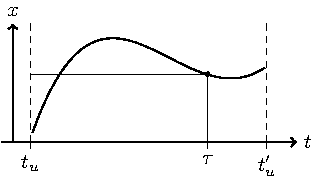
\includegraphics[width=0.5\textwidth]{fig/measurement.pdf}
\caption{
A unit $u$ of type $U$ exists from $t_u$ to $t'_u$. From $t_u$
onward it has an attribute $X$ with its value $x$ possibly changing over time.
At some time $\tau$ this value is observed. The observed value is thus fully
characterized by the quartet ($U$, $\tau$,$u$, $X$).
}
\label{fig:measurement}
\end{figure}
%
A data point usually represents the value of an attribute of an object or event
in the real world: a person, a web site, an e-mail, a radio broadcast, a
country, a sensor, a company, or anything else that has observable attributes.
In what follows, an object or event is referred to as a `unit' for brevity.  A
data point is created by observing an attribute $X$ from a unit $u$ of a
certain type $U$ at time $\tau$, as in Figure~\ref{fig:measurement}. Using the
same reasoning as above,  this yields a $2^4=16$-way classification of
validation rules: for each element $U$, $\tau$, $u$, $X$ a validation rule
requires a single or multiple instances to be evaluated. However, there are some
restrictions.  Any unit $u$ can only be of one type. So evaluating a validation
rule will never require multiple types and a single unit. Second, the type of a
unit fixes its properties. So a validation rule will never need a single
variable for multiple types. With these restrictions considered, the number
of possible classes of validation rules reduces from sixteen to ten.

To distinguish the classes the following notation is introduced. For each
element $U$, $\tau$, $u$, $X$ assign an $s$ when a validation rule pertains to
a single value of that element and assign an $m$ when a validation rule
pertains to multiple values of that element.  For example, a validation rule of
class $sssm$ needs a single type, a single measurement, a single object and
multiple variables to be evaluated. 

The ten possible classes can themselves be grouped into \emph{validation levels},
according to whether a class is labeled with no, one, two, three, or four
$m$'s.  A higher validation level indicates that we need a larger variety of
information in order to evaluate the rule. The classification, and their
grouping into validation levels is summarized in Table~\ref{tab:validationlevels}.

\begin{table}[h]
\caption{The ten possible classes of validation rules, grouped into `validation
levels'.  A higher level indicates that a wider variety of information is
necessary to evaluate a validation rule.}
\label{tab:validationlevels}
\centering
\begin{tabular}{@{}ccccc@{}}
\multicolumn{5}{c}{Validation level}\\
\hline
0 & 1 & 2 & 3 & 4\\
\hline
ssss & sssm & ssmm & smmm & mmmm \\
     & ssms & smsm & msmm &      \\
     & smss & smms &      &      \\
\hline
\end{tabular}
\end{table}



%

Going from level 0 to 4 corresponds to a workflow that is common in
practice. One starts with simple tests such as range checks.  These are of
level zero since a range check can be performed on a single data point. That
is, one only needs a value that corresponds to a single type, measurement,
unit, and variable.  Next, more involved checks are performed, for instance,
involving multiple variables ($sssm$, e.g. the ratio between two properties of
the same unit must be in a given range), multiple units ($ssms$, e.g.  the mean of
a variable over multiple units must be within a specified range), or multiple
measurements ($smss$, e.g.  the current value of the property of a unit cannot
differ too much from a past value of the same property of the same unit).
Going up in level, even more complex rules are found until rule evaluation
involves multiple variables of multiple units of multiple types measured at
multiple instances ($mmmm$). 

This classification also has an immediate interpretation for data stored in a
data base that is normalized in the sense of \citet{codd1970relational}. In
such a data base, records represent units, columns represent variables, and tables
represent types. The `time of measurement' is represented as a variable as
well. The classification indicates whether a rule implementation needs to
access multiple records, columns or tables.



%%%%%%%%%%%%%%%%%%%%%%%%%%%%%%%%%%%%%%%%%%%%%%%%%%%%%%%%%%%%%%%%%%%%%%%%%%%%%%
\section{Properties of validation rule sets}
Definition~\ref{def:validationrule} implies that a validation rule is a
predicate over a data set that is not a tautology nor a contradiction. This
means that combining two validation rules with $\land$ or $\lor$ does not
automatically yield a new validation rule.  Consider for example the rules
$x\geq 0$ and $x \leq 1$ (using shorter notation for brevity). The rule $x \geq
0 \lor x\leq 1$ is a tautology.  The rule $x \geq 0 \land x\leq -1$ is a
contradiction. In fact, the only operation that is guaranteed to transform a
validation rule into another validation rule is negation.

The fact that validation rules are not closed under conjugation ($\land$) or
disjunction ($\lor$) has practical consequences. After all, defining a set of
validation rules amounts to conjugating them together into a single rule since
a data set is valid only when all validation rules are satisfied. A set of
rules may be such that their conjugation is a contradiction.  Such a rule set
is called \emph{infeasible}. More subtle problems involve unintended
consequences, including \emph{partial infeasibility} \citep{bruni2012formal},
and introduction on fixed values or range restrictions. Other problems involve
the introduction of several types of redundancies \citep{dillig2010small,
paulraj2010comparative}, which make rule sets both harder to maintain and
hamper solving problems such as error localization \citep{bruni2005error,
jonge2019errorlocalization}. In the following, some examples of unintended
effects and redundancies are discussed.  The examples shown here are selected
from a more extensive discussion in \citet[Chapter 8]{loo2018statistical}.  For
simplicity of presentation the rules are expressed as simple clauses,
neglecting the key-value pair representation.

Partial inconsistency is (often) an unintended consequence implied by a pair
of rules. For example the rule set
\begin{align*}
gender &= \str{male} \Rightarrow income > 2000\\
gender &= \str{male} \Rightarrow income < 1000,
\end{align*}
is feasible, but it can only be satisfied when $gender\not=\str{male}$.  Thus,
the combination of rules (unintentionally) excludes an otherwise valid gender
category. 

A simple redundancy is introduced when one rule defines a subset of valid
values with respect to another rule. For example if $x \geq 0$ and $x\geq 1$,
then $x\geq 0$ is redundant with respect to $x\geq 1$. More complex cases arise
in sets with multiple rules. A more subtle redundancy, called `nonrelaxing clause'
occurs in the following situation.
\begin{align*}
x \geq 0 \Rightarrow y \geq 0\\
x \geq 0.
\end{align*}
Here, the second rule implies that the condition in the first rule must always
be true. Hence the rule set can be simplified to 
\begin{align*}
y \geq 0\\
x \geq 0.
\end{align*}
Another subtle redundancy, called a `nonconstraining clause' occurs in
the following situation.
\begin{align*}
x > 0 &\Rightarrow y > 0\\
x < 1 &\Rightarrow y > 1
\end{align*}
Now, letting $x$ vary from $-\infty$ to $\infty$, the rule set first implies
that $y>1$. As $x$ becomes positive, the rule set implies that $y>0$ until $x$
reaches $\infty$. In other words, the rule set implies that $y$ must be
positive regardless of $x$ and can therefore be replaced with
\begin{align*}
y > 0\\
x < 1 &\Rightarrow y > 1
\end{align*}
Methods for algorithmically removing such issues and simplifying rule sets have
recently been discussed by \cite{daalmans2018constraint}, and have been
implemented by \citet{jonge2019validatetools}. In short, the methods are based
on formulating Mixed Integer Programming (MIP) problems and detecting their
(non)-convergence after certain manipulations of the rule sets. General theory
and methods for rule manipulation have also been discussed by
\citet{chandru1999optimization}  and \citet{hooker2000logic} in the context of
optimization.

\section*{Where are we?}
We have seen that data validation (checking data) can be formally defined in
terms of logical statements (predicates) over a data set. Equivalently, we can
define it as a function that accepts a data set and takes values in
$\{\nay,\yay\}$. It is possible to define a very general classification of
validation rules, based on a generic decomposition of the metadata. Combining
validation rules into a set can lead to subtle and unintended consequences that
can be solved in some cases with algorithmic methods.

\section{Exercises}
\label{sect:exvalidation}

\begin{enumerate}
\item In September 2018 we ask the two Dutch citizens Alice and
      Bob the following questions.
  \begin{description}
    \item $X$: Do you have a job? (\texttt{yes}, \texttt{no})
    \item $Y$: What is your age? (\texttt{under-aged}, \texttt{adult}, \texttt{retired})
  \end{description}
  \begin{enumerate}
    \item Describe the domain $D$
    \item Give all values of $k$ (this constitutes $K$)
    \item What is the size of $D^K$? That is, how many data sets are possible?
  \end{enumerate}

\item Using the same case as in the previous exercise, we now restrict the
      possible data sets by approving only data points
      that satisfy the following restrictions.
\begin{description}
\item $job \in\{\texttt{yes},\texttt{no}\}$
\item $age\in\{\texttt{under-aged},\texttt{adult},\texttt{retired}\}$
\item $job=\texttt{yes}\Rightarrow age = \texttt{adult}$
\end{description}
How many data sets are now possible?

\item Decide and explain for the following cases whether it describes a validation 
function or not.
  \begin{enumerate}
  \item 
    $$
    v(x) = \left\{\begin{array}{l}
    \texttt{TRUE} \textrm{ if } x \geq 3 \textrm{ and } x \geq 5 \\
    \texttt{FALSE} \textrm{ otherwise}
    \end{array}
    \right.
    $$
  \item 
    $$
    v(x,y) = \left\{\begin{array}{l}
    \texttt{TRUE} \textrm{ if } x + y = 3\textrm{ and } x-y = 0\textrm{ and }x \leq1\\
    \texttt{FALSE} \textrm{ otherwise}
    \end{array}
    \right.
    $$
  \item
    $$
    v(x) = \left\{\begin{array}{l}
    \texttt{TRUE} \textrm{ if } x \leq 10 \textrm{ or } x \geq 3\\
    \texttt{FALSE} \textrm{ otherwise}
    \end{array}
    \right.
    $$
  \end{enumerate}

  \item Classify the following rules according to their complexity
        (Table~\ref{tab:validationlevels}).
    \begin{enumerate}
      \item
      $$
      \frac{\textrm{mean}(price_{2018})}{\textrm{mean}(price_{2017})} \leq 1.1  
      $$

      \item
      $$
      \textrm{mean}(price) \geq 1  
      $$

      \item
      $$
      \max\left(
      \frac{x}{\textrm{median}(X)},\frac{\textrm{median}(X)}{x}
      \right) < 10
      $$

      \item The following rule is the fundamental equation for National Accounts
      $$
      \underbrace{COE + GOS + GMI + T_{P\&M} - S_{P\&M}}_{\textrm{GDP, Income approach}} = 
      \underbrace{C + G + I + (X - M)}_{\textrm{GDP, expenditure approach}}
      $$
      where
      \begin{description}
        \item $COE$: Compensation of employees
        \item $GOS$: Gross operating surplus
        \item $GMI$: Gross mixed income
        \item $T_{P\&M}-S_{P\&M}$: Taxes minus subsidies on production and import
        \item $C$: Consumption by households
        \item $G$: Government consumption and investment
        \item $I$: Gross private domestic investment
        \item $X-M$: Export minus Imports of goods and services
      \end{description}
    \end{enumerate}
  \item This is a lab assignment using R. Load the \code{validate} package and load the 
   \code{SBS2000} dataset. 
   \begin{verbatim}
     library(validate)
     data(SBS2000)
   \end{verbatim} 
   This dataset represents a number of records from the
   Structural Business Survey (SBS).
   If you do not have \code{validate} installed, you can install it once using
  \begin{verbatim}
    install.packages("validate")
  \end{verbatim}
  \begin{enumerate}
    \item Read the help file of the dataset: \code{?SBS2000}.
    \item Work through the introductory example of the `data validation cookbook' \code{vignette("cookbook", package="validate")}
    \item Create a new textfile
    \item Define at least 10 rules for the \code{SBS2000} dataset
    \item Provide rationales in comments
    \item Read, and \code{confront()} rules with data
    \item Summarize and plot the results.
    \item Use \code{as.data.frame} and \code{View} to convert and display the results.
    \item Make a \code{plot} of the \code{validator} object.
    \item (Bonus) If you are familiar with \code{rmarkdown}: create a data quality report.
  \end{enumerate}

\item Find an implied rule for the following rule set.
  \begin{verbatim}
      turnover >= 0
      other.rev >= 0
      turnover + other.rev == total.rev
  \end{verbatim}
\item What are the allowed ranges for \emph{age} and \emph{income} implied by
the following rule set?
  \begin{verbatim}
      age >= 18
      if (job == TRUE) age <= 70
      if (income > 0) job == TRUE
      income >= 0
  \end{verbatim}
Try doing it first by hand. Verify your answer using the \code{validatetools} R package
with the function \code{detect\_boundary\_num()}.
\item Simplify the following rule set.
  \begin{verbatim}
    if ( income > 0 ) age >= 16
    age < 12
  \end{verbatim}
Try doing it first by hand. Verify your answer using the \code{validatetools} R package
with the function \code{simplify\_conditional()}.
\item Which of these rules can be left out?
  \begin{verbatim}
    age >= 18
    age >= 12
  \end{verbatim}
Try doing it first by hand. Verify your answer using the \code{validatetools} R package
with the function \code{remove\_redundancy()}.
\end{enumerate}

\hfill{}Check your answers on page~\pageref{sect:ansvalidation}.




\chapter{Relational data}
\label{sect:relational}
Much of the well-structured data used in statistical organizations is stored in
the form of \emph{records}, more formally called \emph{relations}. This Chapter
gives a brief introduction to classical relational database theory.


\section{Relations}
The basic concept underlying classical databases is the idea of a combination
of values, called a \emph{tuple} that are related to one another. The relation
between the values consists of the fact that they are pertain to the same
entity. As an example consider the following tuple.
\begin{equation}
(Id=1, Name="Alice", Age=7, Owns=\{puzzle, bicycle\}).
\label{eq:alice}
\end{equation}
This tuple describes several attributes of a real-world person.  In this case,
the tuple holds the name of a 7 year old person called Alice, who owns a
bicycle and a puzzle.
\begin{terminology}{Tuple}
A \emph{tuple} is a combination of values $(x_1, x_2,\ldots, x_p)$ that take
values in predefined domains.
\end{terminology}
We have introduced a bit of terminology here that needs to be made more precise
for the coming discussion. First of all, we introduced the term \emph{entity}.
An entity is a particular object or event in the real world.  An example of a
real-world entity is \emph{Willem-Alexander Claus George Ferdinand, King of the
Netherlands, Prince of Oranje-Nassau, Squire of Amsberg}.  Each entity is of a
certain \emph{entity type}. The entity type describes all entities that that
belong to a certain group. What constitutes an entity type is in practice
largely a matter of choice. For example we could think of the entity type
`people living in the Netherlands', and define it as `any person who is
registered to live in a Dutch municipality'. Under this condition
\emph{Willem-Alexander Claus George Ferdinand, King of the Netherlands, Prince
of Oranje-Nassau, Squire of Amsberg} is indeed of entity type `people living in
the Netherlands`. Sometimes this is also expressed by saying that
\emph{Willem-Alexander Claus George Ferdinand, King of the Netherlands, Prince
of Oranje-Nassau, Squire of Amsberg} is an \emph{instance} of the type `people
living in the Netherlands`.
%
\begin{terminology}{Entity and Entity Type}
An \emph{entity type} defines a population of entities. An entity
is a real-world object or event. If an entity belongs to a certain
entity type, we say that it is an \emph{instance} of this type.
\end{terminology}

Entities are characterised by their properties. In database-language these are
called \emph{attributes} while statisticians call them \emph{variables}.  It is
important to realize that entities of the same type share an attribute set. For
example, every `person living in the Netherlands' has a `municipality of
residence', namely the municipality where they are registered. Some persons
living in the Netherlands may also own a house on a Greek peninsula. But since
this is not true for all persons living in the Netherlands, the attribute `size
of house on Greek peninsula' is not an attribute for this entity type.
\begin{terminology}{Attribute}
An attribute is a property associated with an entity.  If two entities are of
the same type, they have the same set of attributes, possibly with different
attribute values.
\end{terminology}

This example highlights another common principle: entity types are usually
defined by starting with a broad type and then fixing one or more attributes.
For example, we can start with the entity type `person' and fix the attribute
`municipality' to municipality in the Netherlands. There is one other way of
defining an entity type, and that is by simply listing the entities that belong
to the type. For example, one may define the entity type of `All People with
Dutch Nationality in 2017` by giving a list of all Dutch Social Security
numbers that existed in 2017.


\section{Normalization}
A relational database stores collections of similar tuples.  Normal people call
such a collection a Table, but database theorists call this a \emph{Relation}.
\begin{terminology}{Relation}
A \emph{relation} is a set of tuples, where all tuples have attributes in the
same domains, in the same order.
\end{terminology}
For two tuples (normal people call them records) to be in the same relation,
they must have the same number of attributes and those attributes must be of
the same data type. There are generally several ways of distributing the same
information over relations and tuples in a database. For example, the
information about Alice in Equation~\eqref{eq:alice} can also be represented as a set of
tuples, like so.
\begin{equation}
\begin{array}{l}
(Id=1, Name=``Alice'')\\
(Id=1, Age=7)\\
(Id=1, Owns = \{puzzle, bicycle\}).
\end{array}
\end{equation}

The choice of representation depends on the intended purpose, as also discussed
in Section~\ref{sect:faces}. Historically, focus has been on properties that
were important for business administration systems. Exemplary applications that
drove the development of early database theory are financial and logistic
databases where possibly many users can simultaneously add, remove, or update
data.  An example to keep in mind is a company that buys, sells, and stores
goods at multiple locations.  There are tables of product availability and
location, tables of sales and purchases (transactions) and so on. At any given
time, an employee of the sales department must be able to see whether there is
enough in stock for their next order. A widely applied approach to normalizing
databases was presented in a seminal paper by \citet{codd1970relational}. In
this approach, three levels of database normalization are defined which are
still very much in use today.


\subsection{First normal form}
The idea of the first normal form is to make tuples as simple as possible.
Remember that a tuple is a combination of values, coming from predefined domains.
Another way of expressing this, is to say that the data types of the values in
a tuple must be fixed beforehand. In principle, data types can be very
complex. For example a calendar date is specified by a year, month, and day
(and a time zone which we ignore here) . 
\begin{align*}
(Name =\code{"Alice"}, Birthday = (Year=1991,Month=05,Day=13") )
\end{align*}
So here, the value of $Birthday$ is also a tuple. The domain of $Birthday$
consists of all triples in $\mathbb{N}\times\mathbb{N}\times\mathbb{N}$ that
represent a valid calendar date when their elements are interpreted
respectively as year, month and day.  The first normal form is all about making
tuples as simple as possible, by not allowing data types that are composed of
simpler types.
%
\begin{terminology}{First normal form (1NF)}
A relation is said to be in first normal form (1NF) when:
\begin{itemize}
  \item All tuples have values from the same domains, in the same order. 
  \item There are no duplicate tuples in a relation.
\end{itemize}
\end{terminology}
It is worth noting that there is no intrinsic ordering of tuples (records) in a
relation. This means that in general you can not assume records to be sorted in
any particular way in a database except if you explicitly sort them.

Continuing with the example, we can store Alice's birthday as
$$
(Name =\code{"Alice"}, Birthday = \code{"19910513"} )
$$
The main advantage of 1NF is that operations on the level of relations, like
searching, filtering and sorting are easier to reason about compared to the
situation where tuples might contain complex data values.


The definition of 1NF does raise the question of when something is
\emph{atomic}.  In practice this usually means either a string, a predefined
categorical variable, a Boolean, or a number type such as integer or double
precision, or a date/date-time type.

From a mathematical point of view the idea of atomicity is more subtle. A data
type is atomic only under the set of operations that leave it intact (see also
the definition of algebraic closure in Chapter~\ref{sect:faces}). To clarify
this let us discuss an physical example. In chemistry, atoms and molecules (and
some of their ions) form the 'data type' under chemical reactions.  Which ever
chemical reaction you perform, you can never produce a particle that is not
either an atom (ion) or a molecule. So the set of atoms, molecules and their
ions are closed under chemical reactions. If we allow other, non-chemical
operations, like nuclear fission, we can create particles that are not in the
periodic system, like neutrons, or neutrinos. This shows that the meaning of
`atomic' depends on the operations that you allow. 

Similar to the atoms and molecules in chemistry, we could allow operations on
an \code{Integer} type in a database, other than the familiar arithmetic
operations. For example by pulling them apart into separate bytes, or bits
even. The moral of the story is that there is no absolute definition of
atomicity when it comes to \emph{atomic domains}. In practice, the atomic types
are the simplest data types offered by a programming language or database
system.


%%%%%%%%%%%%%%%%%%%%%%%%%%%%%%%%%%%%%%%%%%%%%%%%%%%%%%%%%%%%%%%%%%%%%%%%%%%%%%%
\subsection{Second normal form}
The intuition behind second normal form, or 2NF in short, is to reduce the
amount of redundancy in storing information and to guarantee a certain
simplicity for each relation. The explicit definition sounds a bit more formal and
requires some explanation.
\begin{terminology}{Second normal form (2NF)}
A relation is said to be in second normal form (2NF) when 
\begin{itemize}
\item it is in 1NF
\item it has no partial dependencies.
\end{itemize}
\end{terminology}
To understand this definition, we need to understand what \emph{partial
dependencies} are. To do so, suppose we have a database with the following
relations.
\begin{center}
\begin{tabular}{|cccc|}
\multicolumn{4}{l}{Ownership}\\
\hline
PersonId & ProductId  & Nr & Shop           \\
\hline
1  &   107   &2  & Toy store \\
1  &   101   &1  & Bicycle store\\
2  &   104   &1  & Toy store\\
\hline
\end{tabular}
$\:\:$\begin{tabular}{|cc|}
\multicolumn{2}{l}{Products}\\
\hline
Id  & Product \\ 
\hline
101 & bicycle\\
104 & ball   \\
107 & puzzle \\
\hline
\end{tabular}$\:\:$\begin{tabular}{|ccc|}
\multicolumn{2}{l}{Persons}\\
\hline
Id  & Name & Age \\ 
\hline
1 & Alice & 7\\
2 & Bob   & 6\\
\hline
\end{tabular}
\end{center}
In the first relation, the key `PersonId' identifies a person whose properties are
stored in the third relation, while the key `ProductId' identifies an object in the
second relation. Together, these two keys completely identify how many objects
of a given type each person owns. For example, we can ask: `how many puzzles
does Alice own?' and look up that information by finding the key combination
$(\textrm{Id}=1, \textrm{Object}=107)$ in the relation `Ownership'.  Compare this
with the situation for the `Shop' attribute. The value of `Shop' does not
depend on `PersonId` and `ProductId`, but only on `ProductId`. One could say that it is
over-identified, or in data-base terminology it only \emph{partially depends}
on the keys available in the relation.  We can improve this situation by moving
the `Shop` variable to the `Products' relation.
\begin{center}
\begin{tabular}{|ccc|}
\multicolumn{3}{l}{Ownership}\\
\hline
PersonId & ProductId  & Nr   \\
\hline             
1  &   107   &20     \\
1  &   101   &5     \\
2  &   104   &3     \\
\hline
\end{tabular}$\textrm{ }$\begin{tabular}{|ccc|}
\multicolumn{3}{l}{Products}\\
\hline
Id  & Product & Shop          \\ 
\hline                       
101 & bicycle& Bicycle store     \\
104 & ball   & Toy store \\
107 & puzzle & Toy store     \\
\hline
\end{tabular}$\textrm{ }$

\begin{tabular}{|ccc|}
\multicolumn{2}{l}{Persons}\\
\hline
Id  & Name & Age \\ 
\hline
1 & Alice & 7\\
2 & Bob   & 6\\
\hline
\end{tabular}
\end{center}
Now none of the relations have attributes with partial dependencies, which
brings them in second normal form. Of course, we do see that there is some
redundancy in data storage since we have some duplicates for the `Shop`
variable. This will be remedied in the third normal form. But before we get to
that, we need to discuss something about keys.

As you may have noticed, we silently introduced the term `key' into the
discussion.  In real-world databases, each and every tuple (record) is uniquely
identified by an explicitly defined key or combination of keys. Such a key is
usually an otherwise meaningless number that carries no information except the
identity of the entity that is described by the tuple. Examples include social
security and passport document number. When a single key identifies each tuple,
this is called the \emph{primary key}. If no such key is provided by the
database designer, database software will typically create one in the
background, possibly invisible to the user. In formal database theory however,
there is no concept of key as a special kind of attribute. In formal theory one
works with sub-tuples, called \emph{candidate keys} that uniquely identify the
other values in the tuple. For a given relation, there may be multiple
candidate keys, with different numbers of attributes in them. This level of
abstraction makes database theory more general but also more cumbersome to
discuss, which is why they we do not discuss it here.


%%%%%%%%%%%%%%%%%%%%%%%%%%%%%%%%%%%%%%%%%%%%%%%%%%%%%%%%%%%%%%%%%%%%%%%%%%%%%%%
\subsection{Third normal form}
The intuition behind the third normal form is again fairly easy to state.  To
avoid duplication of information, store tuples that represent different entity
types in different relations. Continuing with the example of the previous
paragraph, we see that in the second relation, values of the attribute `Shop'
are duplicated in the second relation. Now suppose we want to change 'Toy
store' into `Department store'. For data in this form we need to update two
fields in the second relation. We can solve this by creating a fourth relation
with different `Shops'.  The result is a set of relations that are interlinked
by shared keys, without data duplication.
%
\begin{center}
\begin{tabular}{|ccc|}
\multicolumn{3}{l}{Ownership}\\
\hline
PersonId & ProductId  & Nr   \\
\hline             
1  &   107   &20     \\
1  &   101   &5     \\
2  &   104   &3     \\
\hline
\end{tabular}
$\textrm{ }$\begin{tabular}{|ccc|}
\multicolumn{3}{l}{Products}\\
\hline
Id  & ProductId & ShopId         \\ 
\hline                       
101 & bicycle& S2     \\
104 & ball   & S1 \\
107 & puzzle & S1     \\
\hline
\end{tabular}$\textrm{ }$\begin{tabular}{|ccc|}
\multicolumn{3}{l}{Persons}\\
\hline
Id  & Name & Age \\ 
\hline
1 & Alice & 7\\
2 & Bob   & 6\\
\hline
\end{tabular}$\:\:$\begin{tabular}{|cc|}
\multicolumn{2}{l}{Shops}\\
\hline
Id  & Shop   \\ 
\hline
S1 & Toy Store \\
S2 & Bicycle Store\\
\hline
\end{tabular}
\end{center}
Now, if we update the label `Toy store' to `Department store' it only needs to
be done in a single attribute of a single tuple in a single relation, and all
queries on this set of relations done afterwards must return the new label.


We are now ready to move on to the formal definition of the third normal form.
\begin{terminology}{Third normal form (3NF)}
A relation is said to be in third normal form when
\begin{itemize}
\item it is in 2NF
\item there are no non-prime attributes that are transitively dependent on a key.
\end{itemize}
\end{terminology}
A non-prime attribute is an attribute that is not a key or part of a set of
attributes that together form a key (that is, a set of attributes that uniquely
identify each record). This non-primality condition is really just theoretical
fine-print. It is necessary to define 3NF without explicitly assuming that one
of the attributes in a relation is an identifying variable.  In databases we
always do have such a variable, so we'll use that in the example. The key
concept in the definition is \emph{transitive dependency}.  We have seen what a
dependency is: the value of variable $X$ determines what the value of variable
$Y$ must be. We can denote this with $X\to Y$. For example in the the following
table we have $\textrm{Id}\to \textrm{Object}$.
\begin{center}
\begin{tabular}{|ccrc|}
\multicolumn{4}{l}{Products}\\
\hline
Id  & Product & Price &Shop          \\ 
\hline                       
101 & bicycle& 250,00 &Bicycle store     \\
104 & ball   & 3,50   &Toy store \\
107 & puzzle & 5,00   &Toy store     \\
\hline
\end{tabular}
\end{center}
Such a dependency is called a \emph{functional dependency}. To be precise, the
notation $X\to Y$ means that `whenever two tuples have the same value for
$X$, they have the same value for $Y$. It follows that if we have $X\to Y$ and
we have $Y\to Z$ then this must imply $X\to Z$. This is called the
\emph{transitive property} of functional dependencies.

Now let's take a look at the above table. We have $\textrm{Id}\to
\textrm{Product}$, but we also have $\textrm{Product}\to\textrm{Shop}$.
Namely, for any two Objects that are the same, we have the same Shop (observe
that the converse is not true). This is
trivial here, since every `Product' occurs only once, but nevertheless we see
that
$$
\textrm{Id}\to\textrm{Product}\textrm{ and }\textrm{Object}\to\textrm{Shop}
$$
and therefore we must have the transitive dependency
$$
\textrm{Id}\to \textrm{Shop}.
$$
In other words, the shop type depends indirectly on the identifying key for
`Product'. 

Bringing a relation into third normal form amounts to bringing it first into
second normal form, and then identify the attribute or attributes that show
transitive dependence on other (sets of) attributes. The transitively dependent
attributes are then moved to a separate table.


Any database can in principle be automatically put into 3NF, although in
general there may be more than one solution and some steering based on domain
knowledge is likely to be necessary.  For example, we see in the example
that `Price' also transitively depends on `Id' even though in reality it
is an attribute of a `Product'. In practice, databases are designed by
information analysts and database administrators to be in third normal form in
the first place.  And this brings us to the topic of the next section. 



%%%%%%%%%%%%%%%%%%%%%%%%%%%%%%%%%%%%%%%%%%%%%%%%%%%%%%%%%%%%%%%%%%%%%%%%%%%%%%%
\section{Entity-Relationship diagrams}
\label{sect:erd}
The basic recipe for designing a particular database structure sounds deceivingly
simple:
\begin{enumerate}
\item Identify all the entity types and their properties.
\item Create relations with tuples of the form
$$
(Id, Property_1, Property_2,\ldots,Property_n),
$$
where $Id$ is a \emph{primary key}.
\item A connection between two entities of different entity types is
represented as a relation that contains the primary keys of both entities.
\end{enumerate}

In practical situations, the number of entity types can grow quickly.  Consider
again as an example the situation of Alice and Bob, who own a few objects, that
were bought in a few stores. We've seen that in 3NF there are three obvious
entity types involved, namely `Person' (Alice and Bob), `Object' (bicycle,
ball, puzzle), and `Shop'. Moreover there is an entity type that expresses an
`Ownership' relation between `Person' and `Object'. This is an entity type
because it has unique properties that can not be attributed to a person or
object alone. Here it is only the Size of the ownership (`Nr'), but we can also
think of a starting and ending time of ownership as relevant attributes of this
relation.

Because relations and their interconnections tend to quickly gain complexity,
their design is usually represented graphically in something called an
\emph{entity-relationship diagram} (ERD). As an example, consider the ERD of
the Alice and Bob example in Figure~\ref{fig:erd}.
\begin{figure}[h]
\centering
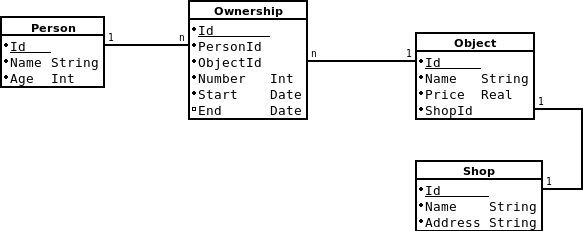
\includegraphics[width=\textwidth]{fig/alice_bob.png}
\caption{Entity-Relationship diagram of people owning objects
bought in shops for a certain price.}
\label{fig:erd}
\end{figure} 
In this diagram, each entity type and its properties are represented in a box.
In this case we also added the type of each property, and labeled the unique
identifier with an asterisk. Whenever the unique identifier (\emph{primary
key}) of one entity occurs in the table of another entity, this is called a
\emph{foreign key}.  This is indicated with a line between boxes that connects
the primary key of one relation with the foreign key in another relation. The
lines are labeled with the type of relationship. For example, the `Id' of a
Person can occur multiple ($n$) times as a foreign key in the `Ownership'
relation.  Whether a connection between two relations is one-to-one,
one-to-many, or many-to-many is called the \emph{arity} of the connection.
%
\begin{terminology}{Primary key, foreign key}
A primary key is a code that uniquely identifies an entity in the relation
representing that entity type. A foreign key is an identifier of one entity
type that occurs in the relation representing another entity type.
\end{terminology}
%
The entity-relationship diagram shown in Figure~\ref{fig:erd} graphically
represents a simple \emph{database schema}. A database schema is a formal
representation of the structure of a database, this includes choices such as
which relations are there, what data is allowed to enter those relations (and
what not) and what are the interconnections between the relations. There are
many tools available that allow one to specify a schema graphically, as in
Figure~\ref{fig:erd}. The software then creates a formal specification for a
particular database management system (DBMS).
\begin{terminology}{Database schema}
A database schema denotes, in a formal (programming) language the
structure of a database.
\end{terminology}

Over time, many variations of entity-relationship diagrams have been developed.
They differ for example in the way the \emph{arity} of connections are
represented.  In some styles an entity type must always be a noun, while a
relation must always be a verb.  In this paragraph we only highlight the most
important bits, as we will return to more formal information modeling in
Chapter~\ref{sect:uml}. The elements we have discussed here are enough to give
a rough sketch for databases


%%%%%%%%%%%%%%%%%%%%%%%%%%%%%%%%%%%%%%%%%%%%%%%%%%%%%%%%%%%%%%%%%%%%%%%%%%%%%%%
\section{Introduction to relational algebra}
Relational algebra consists of a set of basic operations that combine or alter
relations (sets of similar tuples). The basic operations are very general, and
do not depend on type of database, programming language used, or other
implementation details. In fact there are many implementations of these basic
ideas, an we will discuss two of them at the end of this Section.

But before continuing it is worth spending a few words on why having an
`algebra' is important. Recall that the important property of being algebraic
is to have operations that turn things into other things of the same type. Let
us illustrate this with a little algebra we all know. Consider the following
exercise.
$$
\frac{3\cdot 2 + 3\cdot5}{7}
$$
There are several ways to compute the result. The most straightforward way
is the following.
\begin{enumerate}
\item Compute $3\cdot 2=6$, and store the result as $x$.
\item Compute $3\cdot 5=15$, and store the result as $y$.
\item Compute $x+y=6+15=21$, and store the result as $z$.
\item Compute $z/7=21/7=3$.
\end{enumerate}
In total we have done three additions and one division. However, since we know
the rules of arithmetic we can do things more efficiently as follows.
\begin{enumerate}
\item Rewrite the exercise as
$
{3\cdot(2+5)}/{7}
$
\item Compute $2+5$ and rewrite by substituting the answer. We are left with
$
{3\cdot 7}/{7}
$
\item cross out the 7 in the denominator against the 7 in the numerator,
and we are done.
\end{enumerate}
Here, we only needed to evaluate a single calculation (adding 2 and 5)
explicitly. Thus, by using algebraic properties of addition, multiplication and
division we were able to save on the number of calculations, at the cost of
some rewriting. 

Having an algebra of operations, together with strict rules about their like
execution order, allows one to simplify calculations significantly.  For a
simple calculation as just shown, rewriting may actually take more time than a
straightforward calculation. But when the objects of calculation are possibly
large relations with data rather than a few numbers, this balance is likely to
tilt the other way.  Indeed, database systems will typically optimize
user-defined operations on data by shuffling their order to minimize execution
time, memory usage, or a combination of both.

\subsection{Basic operations}
The basic operations on relations are usually divided into set operations
(remember that a relation is a set of tuples) unary operations, and binary
operations (joins).  The fact that tables are sets is important insofar that it
implies that the relations can not be expected to be ordered in any way. So as
far as relational algebra is concerned, the tables
$$
\begin{array}{|ll|}
\hline
Name & Height\\
\hline
Mary & 167\\
Eddy & 180\\
John & 178\\
\hline
\end{array}
\textrm{ and }
\begin{array}{|ll|}
\hline
Name & Height\\
\hline
John & 178\\
Eddy & 180\\
Mary & 167\\
\hline
\end{array}
$$
are exactly the same. In fact, the tabular representations above should be considered
just as a convenience. In principle we are working with a set of ordered tuples, for
which the standard mathematical notation is
$$
\{(John, 178), (Eddy,180), (Mary, 167)\}.
$$

There are three binary set operations that work on relations with the same
attributes: set Union $A\cup B$, set Difference $A-B$, and set Intersection
$A\cap B$. Below are examples of each operation.

Union (only works for relations with the same attributes).
$$
\begin{array}{|ll|}
\hline
Name & Height\\
\hline
Eddy & 180\\
\hline
\end{array}
\cup
\begin{array}{|ll|}
\hline
Name & Height\\
\hline
Mary & 167\\
John & 178\\
\hline
\end{array}
=
\begin{array}{|ll|}
\hline
Name & Height\\
\hline
Eddy & 180\\
Mary & 167\\
John & 178\\
\hline
\end{array}
$$
Difference (only works for relations with the same attributes).
$$
\begin{array}{|ll|}
\hline
Name & Height\\
\hline
Eddy & 180\\
Mary & 167\\
John & 178\\
\hline
\end{array} 
-
\begin{array}{|ll|}
\hline
Name & Height\\
\hline
Eddy & 180\\
John & 178\\
\hline
\end{array} 
=
\begin{array}{|ll|}
\hline
Name & Height\\
\hline
Mary & 167\\
\hline
\end{array}
$$
Intersection (only works for relations with the same attributes).
$$
\begin{array}{|ll|}
\hline
Name & Height\\
\hline
Eddy & 180\\
Mary & 167\\
John & 178\\
\hline
\end{array} 
\cap
\begin{array}{|ll|}
\hline
Name & Height\\
\hline
Eddy  & 180\\
John  & 178\\
Alice & 192\\
\hline
\end{array}
=
\begin{array}{|ll|}
\hline
Name & Height\\
\hline
Eddy  & 180\\
John  & 178\\
\hline
\end{array}
$$
In principle one of these `basic relations' is redundant since we can write
intersection as a combination of union and difference (see
Exercise~\ref{ex:settheory}). Having these three basic operations is thus more
a matter of convenience than of theoretical minimalism.



Unary operations are operations that act on a single relation. There are three
unary operations: Projection, Selection, and Rename.  The Projection operation
selects zero or more columns from a relation, returning a possibly smaller relation.
It is denoted as $\Pi_{a_1,\ldots,a_p}$ where the subscripts denote what
columns to select. Here's an example.
$$
\Pi_{Name}\;
\begin{array}{|ll|}
\hline
Name & Height\\
\hline
Mary & 167\\
Eddy & 180\\
John & 178\\
\hline
\end{array}
= 
\begin{array}{|l|}
\hline
Name \\
\hline
Mary \\
Eddy \\
John \\
\hline
\end{array}.
$$
The second unary operation is called Selection. It is denoted $\sigma_\phi$, where
$\phi$ is a Boolean proposition (a selection rule) stating a condition on attributes
in the relation.
$$
\sigma_{Height\leq 170}\;
\begin{array}{|ll|}
\hline
Name & Height\\
\hline
Mary & 167\\
Eddy & 180\\
John & 178\\
\hline
\end{array}
=
\begin{array}{|ll|}
\hline
Name & Height\\
\hline
Mary & 167\\
\hline
\end{array}
$$
The last unary operation is called Rename. It is denoted ${\rho_{a/b}}$ where
$a$ is the name of the attribute to be renamed, and $b$ is the new name.
$$
\rho_{Name/FirstName}\;
\begin{array}{|ll|}
\hline
Name & Height\\
\hline
Mary & 167\\
Eddy & 180\\
John & 178\\
\hline
\end{array}
=
\begin{array}{|ll|}
\hline
FirstName & Height\\
\hline
Mary & 167\\
Eddy & 180\\
John & 178\\
\hline
\end{array}
$$

Finally, there are several types of \emph{join} operations that merge two
relations into a single new relation, based on common values in shared
attributes. The most important one is the \emph{natural join}, denoted
with a `bowtie' symbol: $\bowtie$. This merges two
datasets and only keep the records that can be merged.  This is often referred
to as an \emph{inner join}.
$$
\begin{array}{|ll|}
\hline
Name & Age\\
\hline
John & 25\\
Mary & 34\\
\hline
\end{array}
\;\bowtie\;
\begin{array}{|ll|}
\hline
Name & Height\\
\hline
Mary & 167\\
Eddy & 180\\
John & 178\\
\hline
\end{array}
\;=\;
\begin{array}{|lll|}
\hline
Name & Age & Height\\
\hline
John & 25 & 178\\
Mary & 34 & 167\\
\hline
\end{array}
$$
In formal relational algebra, it is assumed that there are no duplicate keys to
merge on. So for example \emph{Mary} will occurs maximally once in each table
on the left-hand-side (recall the definition of 1NF). In practice duplication
can occur, and we will see in the next section how this is dealt with in
implementations.

The \emph{outer join}, merges two tables on shared attributes with common
values, but also keeps the records that can not be matched. Attributes
of one table that have no match with the other one are left empty.

$$
\begin{array}{|ll|}
\hline
Name & Age\\
\hline
John  & 25\\
Mary  & 34\\
Alice & 57\\
\hline
\end{array}
\;\times\;
\begin{array}{|ll|}
\hline
Name & Height\\
\hline
Mary & 167\\
Eddy & 180\\
John & 178\\
\hline
\end{array}
\;=\;
\begin{array}{|lll|}
\hline
Name & Age & Height\\
\hline
John & 25 & 178 \\
Mary & 34 & 167 \\
Alice& 57 &     \\
Eddy &    & 180 \\
\hline
\end{array}
$$

Both the natural join and the outer join are symmetric, that is $A\bowtie
B=B\times A$ and $A\times B=B\times A$ for any two relations $A$ and $B$. There
are also variants that are \emph{not} symmetric. The \emph{left join}, denoted
$\ltimes$, keeps all records from the left hand side and adds records at the
right hand side where possible. Attributes for records with no match are left
empty.

$$
\begin{array}{|ll|}
\hline
Name & Age\\
\hline
John  & 25\\
Mary  & 34\\
Alice & 57\\
\hline
\end{array}
\;\ltimes\;
\begin{array}{|ll|}
\hline
Name & Height\\
\hline
Mary & 167\\
Eddy & 180\\
John & 178\\
\hline
\end{array}
\;=\;
\begin{array}{|lll|}
\hline
Name & Age & Height\\
\hline
John & 25 & 178 \\
Mary & 34 & 167 \\
Alice& 57 &     \\
\hline
\end{array}
$$
Similarly, there is a \emph{right join} denoted $\rtimes$, that keeps all
records of the right hand side. Finally, there is the \emph{antijoin}
operation, denoted $\triangleright$. The antijoin is not really a join
operation. It selects records from the relation on the left-hand side that can
not be matched with the relation on the right hand side.
$$
\begin{array}{|ll|}
\hline
Name & Age\\
\hline
John  & 25\\
Mary  & 34\\
Alice & 57\\
\hline
\end{array}
\;\triangleright\;
\begin{array}{|ll|}
\hline
Name & Height\\
\hline
Mary & 167\\
Eddy & 180\\
John & 178\\
\hline
\end{array}
\;=\;
\begin{array}{|ll|}
\hline
Name & Age\\
\hline
John  & 25\\
Mary  & 34\\
\hline
\end{array}
$$
Observe that the difference between the antijoin and set intersection is that
for set intersection, we demand that the relation on the left hand side has
the exact same attributes as the relation on the right hand side while
this is not the case for antijoin.

To complete our discussion of relational algebra, we need to define the operator
precedence. That is, just like we agreed that in normal arithmetic, multiplication
comes before addition, we need to define the order of execution when combining
multiple relational operations. The order is defined as follows.
\begin{enumerate}
\item $\sigma$, $\Pi$, $\rho$ (highest precedence ---execute this first when possible)
\item $\bowtie$, $\times$, $\ltimes$,$\rtimes$, $\triangleright$
\item $\cap$
\item $\cup$, $-$.
\end{enumerate}
In this booklet we shall always use brackets to make order of execution
absolutely clear.

\subsection{Implementations}
Relational algebra has been implemented, fully or partially in many tools. Here
we shall briefly discuss two of them: SQL and R package `dplyr'. The latter
tool will be used in the workshop exercise. The goal of this chapter is not to
learn how to work with SQL, but to raise awareness that the formal concepts
introduced so far have real and practical implementations that are used every
day.

The most important implementation of relational algebra is SQL, which stands
for Structured Query Language. SQL is in itself not a tool, but the definition
of a programming language that treats tables as a basic type. This programming
language is implemented in many (commercial) database systems where different
vendors typically create their own dialect of SQL, for example by extending it
with certain capabilities for data analyses. However the basic operations
treated here are usually all present.

Here is an example. Suppose we have a table called `A' and we wish to select the attribute
called `Height'. In SQL this would look something like this.
\begin{verbatim}
  SELECT Height FROM A
\end{verbatim}
So here, \code{SELECT HEIGHT} is a direct translation of $\Pi_{Height}$ and the
whole expression means $\Pi_{Height}A$. If we want to do a left join on the
Name attribute between A and B, and subsequently select `Age' and `Height', we
get the following.
\begin{verbatim}
  SELECT Height, Age FROM 
    A LEFT JOIN B ON Name
\end{verbatim}
Observe that the operator precedence discussed in the previous section ensures
that $A\ltimes B$ is computed first and next `Height' and `Age' are selected.
Readers interested in learning SQL could have a look at the online tutorial
of the W3Schools organization\footnote{
\href{https://www.w3schools.com/sql/default.asp}{https://www.w3schools.com/sql/default.asp}
}.

A second --sort of-- implementation comes with R package `dplyr`.  In R, a
relation is represented by something called a \emph{data.frame}.  There are no
ways to force the absence of duplicates, or even atomicity of its contents, so
this data type is more flexible than the type of relations where relational
algebra was designed for. Although R \citep{Rcore} comes with implementations
of all relational operators that work on data frames, many people find the
syntax implemented in the \code{dplyr} package easier to work with, so this is
what we will discuss here.

To select a column called `Height' from a data frame called `A', in
\code{dplyr} one calls a function called \code{select}.
\begin{verbatim}
  select(A, Height)
\end{verbatim}
Since `dplyr` does not offer a programming language, but a set of functions,
some syntax is needed to take the output of one function and pass it to
the next function. Here we use the so-called pipe operator and work out the
second example.
\begin{verbatim}
  A %>% 
    left_join(B, Name) %>%
    select(Height, Age)
\end{verbatim}
Here, the \code{\%>\%} operator takes the output on the left hand side and
feeds it as the first argument of the functions on the right hand side.  This
is equivalent to storing intermediate results and reusing that in the
calculations.
\begin{verbatim}
  X <- left_join(A, B, Name)
  select(X, Height, Age)
\end{verbatim}
Which syntax is preferred is to an extend a matter of taste. The former syntax
with \code{\%>\%} is quicker to develop, the latter syntax is easier to debug
since intermediate results are available.










\subsection*{Where are we?}
We have see that the concepts of tables and records can be treated formally in
database theory, where they are called respectively relations and tuples.  The
formal treatment yields normalized forms that can be described and designed
graphically using entity-relationship diagrams (database diagrams).  Moreover,
there is a small number of basic operations that can be used to manipulate of
sets of relations. Many commonly used tools implement these operations or
variants thereof so they are ubiquitous in data management.


\newpage
%%%%%%%%%%%%%%%%%%%%%%%%%%%%%%%%%%%%%%%%%%%%%%%%%%%%%%%%%%%%%%%%%%%%%%%%%%%%%%%
\section{Exercises}
\label{sect:exrelational}

\begin{enumerate}
\item Put the following table in 1NF

\begin{tabular}{|cccc|}
\hline
Id & Name  & Age & Owns \\
\hline
1  & Alice & 7 & $\{\textrm{puzzle},\textrm{bicycle}\}$\\
2  & Bob   & 6 & $\{\textrm{ball}\}$\\
\hline
\end{tabular}
\item In official statistics, there are several ways to count businesses. There
are `legal units' which are defined by their registration at the Chamber of
Commerce. There are `Tax' units which are defined as one or more legal units
that together file a tax report.  And then there are `Economic units'. These
are constructed by Official Statisticians by combining one or more legal units
into an establishment that coherently conducts its business. Exemplary cases
are large (multinational) companies that separate activities into different
legal units. It is also possible for multiple legal units to form  a new Tax
unit, but those legal units do not necessarily come from the same economic
unit. How would you store such data? Create a database schema to reflect that.
\item Consider the database schema in Figure~\ref{fig:recordschema} and answer
the following questions.
\begin{enumerate}
  \item How many attributes are there in the employees table?
  \item What are the foreign keys in the `tracks' table?
  \item What is the type of the primary key in `customers'?
\end{enumerate}
\begin{figure}[t]
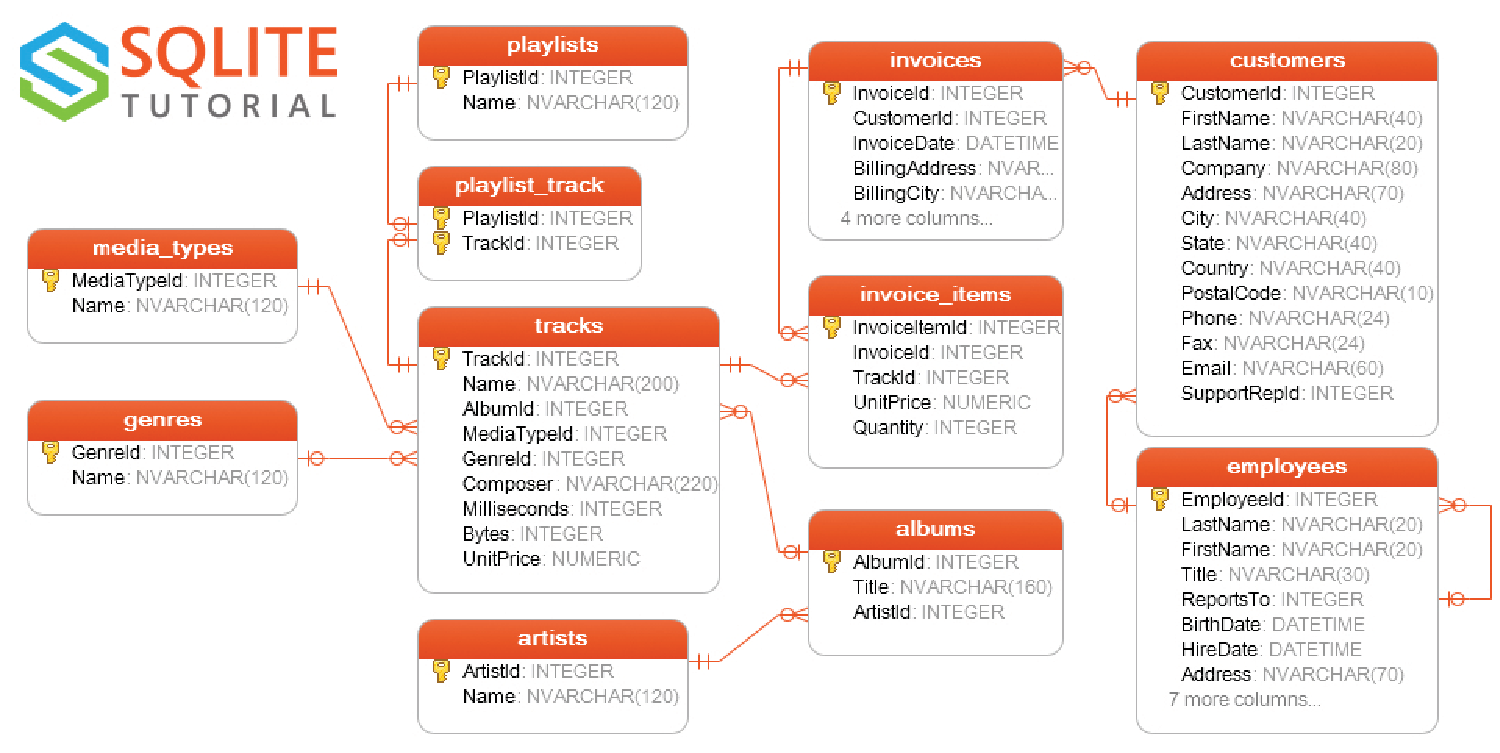
\includegraphics[width=\textwidth]{fig/recordschema.pdf}
\caption{A database scheme for record sales, taken from from the SQLite tutorial 
(\href{sqlitetutorial.net/sqlite-sample-database/}{https://www.sqlitetutorial.net/sqlite-sample-database/}).
}
\label{fig:recordschema}
\end{figure}
\item Create a database schema for the case in Section~\ref{sect:schema}.
\item \label{ex:settheory} Consider the sets $V=\{a,b,c,d,e\}$ and
$W=\{b,d,f\}$.  Show that in this case $V\cap W$ gives the same result as $V\cup W- (V - W)
- (W - V)$. Bonus question: can you prove this is true for any two sets $V$ and $W$?
\item Consider the following two tables.
$$
A =
\begin{array}{|ll|}
\hline
Name & Age\\
\hline
John  & 25\\
Mary  & 34\\
Alice & 57\\
\hline
\end{array}
\;
B = 
\begin{array}{|ll|}
\hline
Name & Height\\
\hline
Mary & 167\\
Eddy & 180\\
John & 178\\
\hline
\end{array}
$$
\label{ex:schema}
Compute the following relations, try to simplify the calculations before
filling in the actual relations.
\begin{enumerate}
  \item $\Pi_{a\in A}(A\ltimes B)$, where $a\in A$ means all attributes occurring in $A$. 
  \item $\sigma_{Age>40} (A\bowtie B)$.
  \item $\sigma_{Age\leq40\land Height\leq 170} (A\times B)$. (The symbol $\land$ means `AND').
  \item $\Pi_{Height}A\bowtie B$.
\end{enumerate}
\item Take a look again at the schema in Figure~\ref{fig:recordschema}. How
would you create the following relations? Use notation from relational algebra
to express this.
\begin{enumerate}
  \item A relation with one tuple for each track, holding Album Title and Track Name.
  \item A relation with Artist, Track, and customerId, so we can identify in what artists
        each customer is interested.
  \item A relation with TrackId and EmployeeId so we can analyze which employee sells most tracks.
\end{enumerate}

\end{enumerate}

\hfill{}Check your answers on page~\pageref{sect:ansrelational}.


\begin{subappendices}
\section{Case: car rentals}
\label{sect:schema}

Your job is to design a database schema for the case below. You can do it on
pen and paper (great to get started!), use a drawing programme, or one of the
many (online) free database schema creators. An example is
\hlink{https://www.dbdesigner.net}{dbdesigner}.  You can use the guest login or
create a free trial account. (Note: you will not be able to save your schema,
but you can export an image or SQL code)\footnote{
This assignment was taken from the Master's Thesis of
\citet{zhang2012suite}.
}.


\subsection*{Part 1}

Our company does car rental business and has several locations with different
address (address consist of street with the number, city, and postal code). In
large cities there can be multiple locations. The cars are classified as
subcompacts, compacts, sedans, or luxury. Each car has a particular model, year
made, and color. Each car has a unique identification number and a unique
license plate.

\subsection*{Part 2}

Cars rented in a particular location may be returned to a different location
(pickup and drop-off). For every car we keep the odometer (km traveled) reading
before it is rented and after it is returned. The car is rented out with full
tank and we record the volume of gas in the tank when the car is returned, but we
only indicate if the tank is empty, quarter full, half full, three quarters
full, or full.

\subsection*{Part 3}

We keep track of which day a car was rented, but not of the time, similarly for
car returning. If a customer requests a specific class (say sedan), we may rent
the customer a higher-class car if we do not have the requested class in the
stock, but we will price it at the level the customer requested (so-called
upgrade). Each car class has its own pricing, but all cars in the same class are
priced the same. 


\subsection*{Part 4}

We have rental policies for 1 day, 1 week, 2 weeks, and 1 month. Thus, if a
customer rents a car for 8 days, it will be priced as 1 week + 1 day. The
drop-off charge only depends on the class of the rented car, the location it was
rented from and the location it is returned to. About our customers, we keep
their names, addresses, possibly all phone numbers, and the number of the
driver’s license (we assume a unique license per person). 

\subsection*{Part 5}

About our employees we keep the same basic information as our customers (we
require that all our employees have a driver’s license). We have several
categories of workers, drivers, cleaners, clerks, and managers. Any of our
employees can rent a car from our company for a 50% discount, if the rental is
less than 2 weeks. However, for any longer rental they must pay 90% of the
regular price. Every employee works in one location only. 

\end{subappendices}




\chapter{Data in organizations}
In this Chapter we discuss some high-level ideas on how databases can be
implemented in an organization. We also discuss one theoretical result that
helps to guide the choice of database implementation.


\section{Data architecture}
Understanding relational database theory and implementations thereof is one
thing. It is another thing entirely to actually use these ideas in production
environments. In practice one needs to make trade-offs between availability,
consistency, flexibility, and database performance. It has to be decided which
users have access to what data, what actions each user is allowed to perform.
For example, a data analyst may only temporarily need read-only access while
data base administrators have the ability to create or delete whole tables.
Especially in larger organisations, one needs to have procedures in place to
decide who is granted what rights, for how long, and on what grounds. 

Since there are many choices to be made, it is advantageous to have a global
overview of all things related to data in an organisation.  Such an overview is
called a 'data architecture'. To be precise, The Open Group on Architecture
Frameworks
(\hlink{https://pubs.opengroup.org/architecture/togaf9-doc/arch/index.html}{TOGAF})
defines a data architecture as follows.

\begin{terminology}{Data Architecture} 
A description of the structure and interaction of the enterprise's major types
and sources of data, logical data assets, physical data assets, and data
management resources. 
\end{terminology}
Architecture documents can describe the state of an organisation as it
currently works, but they can also serve as the design of how an organisation
should work in the future.  The idea is that this helps decision makers across
the organisation to make consistent choices. Nowadays, many large organizations
employ enterprise and data architects. For official statistics, a Common
Statistical Data Architecture was developed under the auspices of the United
Nations initiative on the modernisation of official statistics
(\hlink{https://statswiki.unece.org/display/DA}{CSDA}).

Architectures include a broad range of aspects, ranging from organizational
issues to technical (software) and physical (hardware) choices. 

In this section
we will focus on a few well-known methods for organizing databases.

As long as databases have been used in the industry, people have discussed how
to organize them. Over time, several general ideas on how to structure
databases in an organization have evolved. Many of these ideas have been
developed over time in industry, and the terminology used is not always
consistent. Most of these ideas have first been published in white papers, or
blog posts or other publications that have not been peer reviewed.  However
some of these ideas have become commonplace in industry and it is well worth
taking note of them as they do demonstrate how the theoretical ideas discussed
in Chapter~\ref{sect:relational} end up being used in practice. In the
following subsections we give an overview of some of the most well-known
database architectures, and discuss some of their advantages and disadvantages.

\subsection{Data Warehouse and Data Mart}
The data warehouse is the classical data base architecture. It is designed to
be a \emph{single source of truth} for the whole organization. This means that
the traditional data warehouse typically consists of a single database system
where all data is stored. Data that is sent to the data warehouse has to pass
strict checks before being allowed to enter. Data warehouses are governed and
centrally within an organization. Technically, they are often implemented as
relational databases. 

Data warehouses typically harbour data that is absolutely necessary to run a
business (mission-critical), and that must be consistent across the
organization. In NSIs, sampling frames that are used by various departments
fall under that category. When two sample surveys are to be used to make
inferences about the same population, the samples should be drawn from the same
population register. In businesses, customer administration and human resources
typically also fall under that category.

\begin{figure}[h]
\centering
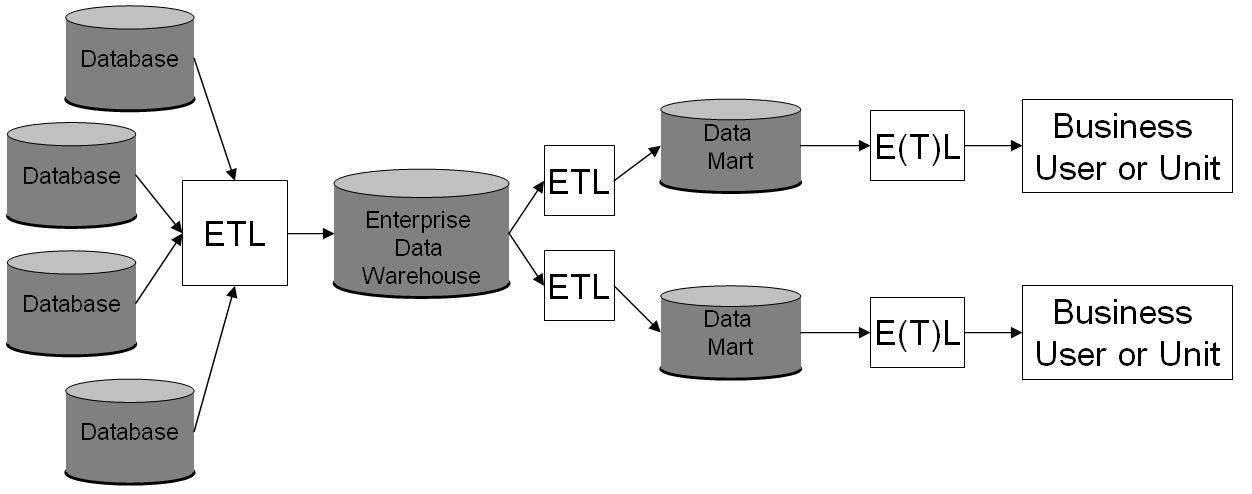
\includegraphics[height=25mm]{fig/data_warehouse_data_mart.jpg}
\caption{A data warehouse, feeding data marts. ETL stands for 
Extraction, Transformation and Loading. Picture from Wikimedia commons.}
\end{figure}

Thus, the advantage of a data warehouse architecture is that data is reliable
and strictly maintained. An immediate disadvantage is lack of flexibility.
With centrally controlled systems it may be cumbersome to create custom tables
for ad hoc analyses, or to add variables or otherwise manipulate the database
schema in ways that are interesting for analyses, since such changes
potentially have consequences in many places in the organization. 

An early answer to this disadvantage is the `data mart' architecture. In this
design, there is a central data warehouse but different users are allowed to
create their own local data bases that combine data from the warehouse with
locally created data. For example, in the case of an NSI a department that
conducts a certain business survey may join that data to a centrally stored
register of tax data and data from the Chamber of Commerce. This way, analysts
have freedom to set up local systems while the `single source of truth' stays
intact. Typical disadvantages of the data mart structure include proliferation
of data base systems and duplication of work.


\subsection{Data Lake}
The idea of a data lake was invented as an answer to the disadvantages caused
by the rigidity of centralized data warehouses. Recall that in a data
warehouse, the data base schemas are strictly controlled and therefore it may
take a lot of effort to condition data for it to be accepted into the database.
Also, as the types of data that are interesting for an organization to harvest
become more diverse and larger, keeping everything in a central data warehouse
becomes more or less impossible to organize.

The term data lake was invented by James Dixon, who wrote a blog post about it
in
\hlink{https://jamesdixon.wordpress.com/2010/10/14/pentaho-hadoop-and-data-lakes/}{2010}.
It was further elaborated upon in a white paper of \citet{stein2014enterprise}. Dixon
summarizes the idea as follows.
\begin{quote}
If you think of a datamart as a store of bottled water ---cleansed and packaged and
structured for easy consumption--- the data lake is a large body of water in a more
natural state. The contents of the data lake stream in from a source to fill the lake,
and various users of the lake can come to examine, dive in, or take samples.
\end{quote}

The idea is to remove the barrier for storing data completely. In a data lake, all
data is stored in a key-value store. Data can in principle be anything, including
documents, images, videos, audio or other formats. There is little organization
in storing the data, except for a unique identifier attached to each item. The main
task of a data lake is to store data so it can in principle be analyzed later. The
technical solution proposed by Dixon is to use a Hadoop-like key value store.

The main disadvantage of a data lake is that data needs to be gathered and
cleaned for every separate task. Having little structure in the data means that
it is hard to automate over and generally it requires more advanced skills to
work with data from a data lake than data from a data warehouse.


\subsection{Data Virtualisation}
In both the data warehouse and data lakes, data is moved from the data source
into a central or distributed database system. This may become cumbersome,
especially for very large and very diverse datasets. In data virtualisation,
data stays at the source, and instead there is a database that stores where
data can be found. Since users may access that database more or less as if it
were a regular database, this is called `data virtualisation`. The data is
retrieved by the `virtualisation' software as needed.

An advantage of data virtualisation is that the technical introduction into an
organization is relatively easy. Hardly any changes are necessary in existing
systems. The main challenges are organisational. For example in the situation
of a data mart, it needs to be decided which local databases must be connected
to the virtualisation software, and how. 



\section{The CAP theorem}
\label{sect:relational:cap}
For large datasets, data that needs to be accessed by many users, or data that
needs to be available at many places simultaneously, it is common to use some
form of distributed database. 
\begin{terminology}{Distributed database}
A distributed database is a database system that is spread over two
or more nodes.
\end{terminology}
%
The term `node' is just a fancy word for a computer in a network, or an
application that runs as if it was on a separate computer in a network. When a
database is running on multiple nodes, there has to be some communication
between the nodes to synchronize information between them. The CAP theorem
demonstrates that there are fundamental limits on what one can expect from such
a system.
%
\begin{terminology}{CAP Theorem}
A distributed database can not simultaneously be Consistent, Available, and
Partition-tolerant.
\end{terminology}
The CAP theorem was conjectured in 2002 by Eric \citet{brewer2002towards} and
proven quickly thereafter by \citet{gilbert2002brewer}.  The original proof is
a bit technical and requires a fair amount of technical definitions.  In the
current discussion we use the visual proof as discussed by
\hlink{https://mwhittaker.github.io/blog/an\_illustrated\_proof\_of\_the\_cap\_theorem/}{Whittaker},
which is easier to follow and captures the main arguments.


First consider a network composed of two nodes, called $G_1$ and $G_2$. The
network hosts a database, and both nodes have access to a stored variable with
value $v_0$.
%
\begin{center}
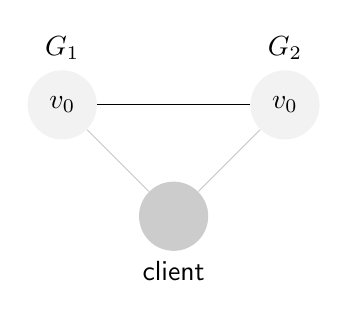
\begin{tikzpicture}[node distance = 2cm]
\tikzstyle{every state} = [fill=shadecolor, draw=none];
\tikzstyle{client} = [state, fill=black!20];
\tikzstyle{clnd} = [-, color=black!20];

\node[state, label=above:$G_1$] (G1) {$v_0$};
\node[client, below right of = G1, label=below:client] (cl) {};
\node[state, above right of = cl, label=above:$G_2$] (G2) {$v_0$};
\path (G1) edge (G2);
\draw[clnd] (cl) to (G1);
\draw[clnd] (cl) to (G2);

\end{tikzpicture}
\end{center}
%
The two nodes can be accessed by a client, that can request each node to return
the current value (a `read' operation) or to overwrite the current value with
another value, say $v_1$.

Now, for the database to be \textit{consistent}, means that 
\begin{quote}
any read operation that begins immediately after a write operation is completed must
return that value.
\end{quote}
The important thing is that this must hold regardless of which nodes are
receiving the read or write request. Here is how the two-node database can be
consistent: it needs to synchronizes before it is done with a `write'
operation.
\begin{center}
%% client sends 1 write request
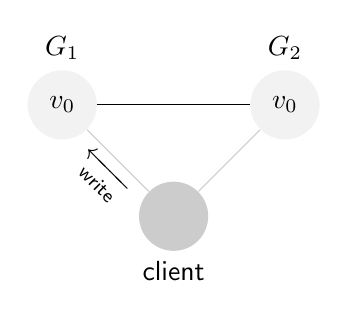
\begin{tikzpicture}[node distance = 2cm]
  \tikzstyle{every state} = [fill=shadecolor, draw=none];
  \tikzstyle{client} = [state, fill=black!20];
  \tikzstyle{clnd} = [-, color=black!20];

  \node[state, label=above:$G_1$] (G1) {$v_0$};
  \node[client, below right of = G1, label=below:client] (cl) {};
  \node[state, above right of = cl, label=above:$G_2$] (G2) {$v_0$};
  \path (G1) edge (G2);
  \draw[clnd] (cl) to node[color=black, sloped, anchor=north, auto=false] 
                      {$\xleftarrow[\textsf{write}]{}$} (G1);
  \draw[clnd] (cl) to (G2);
\end{tikzpicture}
%% node 1 has written, and sends write request
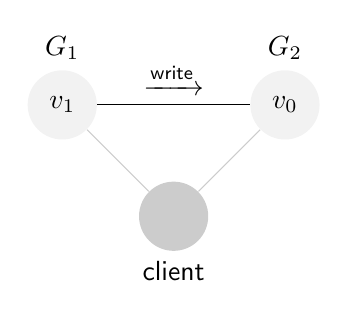
\begin{tikzpicture}[node distance = 2cm]
  \tikzstyle{every state} = [fill=shadecolor, draw=none];
  \tikzstyle{client} = [state, fill=black!20];
  \tikzstyle{clnd} = [-, color=black!20];

  \node[state, label=above:$G_1$] (G1) {$v_1$};
  \node[client, below right of = G1, label=below:client] (cl) {};
  \node[state, above right of = cl, label=above:$G_2$] (G2) {$v_0$};
  \path (G1) edge node[above] {$\xrightarrow{\textsf{write}}$} (G2);
  \draw[clnd] (cl) to (G1);
  \draw[clnd] (cl) to (G2);
\end{tikzpicture}
%% node two has written and sends 'done' signal
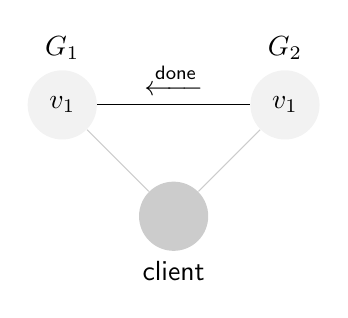
\begin{tikzpicture}[node distance = 2cm]
  \tikzstyle{every state} = [fill=shadecolor, draw=none];
  \tikzstyle{client} = [state, fill=black!20];
  \tikzstyle{clnd} = [-, color=black!20];

  \node[state, label=above:$G_1$] (G1) {$v_1$};
  \node[client, below right of = G1, label=below:client] (cl) {};
    \node[state, above right of = cl, label=above:$G_2$] (G2) {$v_1$};
  \path (G1) edge (G2);
  \path (G1) edge node[above] {$\xleftarrow{\textsf{done}}$} (G2);
  \draw[clnd] (cl) to (G1);
  \draw[clnd] (cl) to (G2);
\end{tikzpicture}
%% node 1 sends 'done' signal to client.
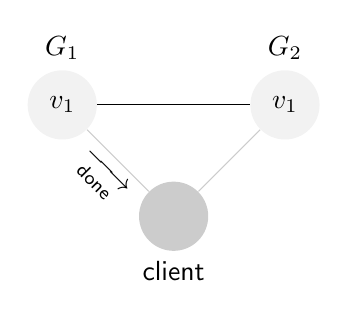
\begin{tikzpicture}[node distance = 2cm]
  \tikzstyle{every state} = [fill=shadecolor, draw=none];
  \tikzstyle{client} = [state, fill=black!20];
  \tikzstyle{clnd} = [-, color=black!20];

  \node[state, label=above:$G_1$] (G1) {$v_1$};
  \node[client, below right of = G1, label=below:client] (cl) {};
  \node[state, above right of = cl, label=above:$G_2$] (G2) {$v_1$};
  \path (G1) edge (G2);
  \draw[clnd] (cl) to node[color=black, sloped, anchor=north, auto=false] 
                      {$\xrightarrow[\textsf{done}]{}$} (G1);
  \draw[clnd] (cl) to (G2);
\end{tikzpicture}
\end{center}
Now the client can read from either node and receive the same answer.
%
\begin{center}
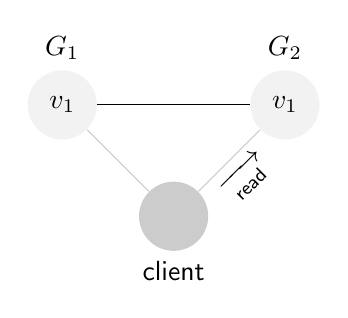
\begin{tikzpicture}[node distance = 2cm]
  \tikzstyle{every state} = [fill=shadecolor, draw=none];
  \tikzstyle{client} = [state, fill=black!20];
  \tikzstyle{clnd} = [-, color=black!20];

  \node[state, label=above:$G_1$] (G1) {$v_1$};
  \node[client, below right of = G1, label=below:client] (cl) {};
  \node[state, above right of = cl, label=above:$G_2$] (G2) {$v_1$};

  \draw (G1) edge (G2);
  \draw[clnd] (cl) to (G1);
  \draw[clnd] (cl) to node[sloped, auto=false, below, text=black] {$\xrightarrow[\textsf{read}]{}$} (G2);

\end{tikzpicture}
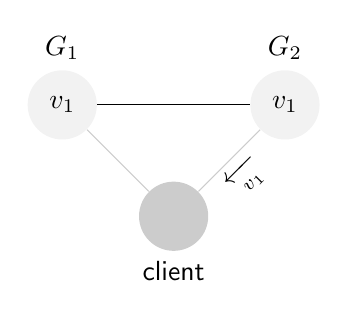
\begin{tikzpicture}[node distance = 2cm]
  \tikzstyle{every state} = [fill=shadecolor, draw=none];
  \tikzstyle{client} = [state, fill=black!20];
  \tikzstyle{clnd} = [-, color=black!20];

  \node[state, label=above:$G_1$] (G1) {$v_1$};
  \node[client, below right of = G1, label=below:client] (cl) {};
  \node[state, above right of = cl, label=above:$G_2$] (G2) {$v_1$};

  \draw (G1) edge (G2);
  \draw[clnd] (cl) to (G1);
  \draw[clnd] (cl) to node[sloped, auto=false, below, text=black] {$\xleftarrow[v_1]{}$} (G2);

\end{tikzpicture}
\end{center}
%

The \emph{availability} demands entails the following.
\begin{quote}
every request received by a non-failing node must result in a response.
\end{quote}
This means that in an available system, if the client sends a request to a node
that is `up' (i.e. not crashed), the node must eventually return a result: nodes 
are not allowed to ignore requests.

Finally, \textit{partition-tolerance} means that
\begin{quote}
the network will be allowed to loose arbitrary many messages sent from one node to
another.
\end{quote}
In particular, partition-tolerance means that the system keeps working even
when one or more nodes are completely separated from the others.

By now, it is probably clear that the CAP theorem must hold: after all, how can
a set of nodes stay synchronized when they can not communicate write requests?
Explicitly, assume that the CAP theorem does hold and consider the situation
where $G_2$ is separated from $G_1$, so no messages can be send in either
direction.
\begin{center}
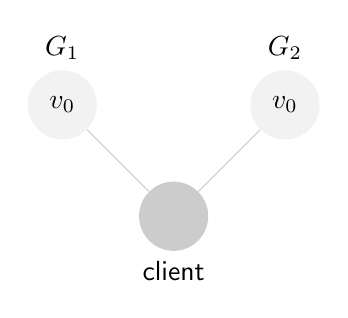
\begin{tikzpicture}[node distance = 2cm]
\tikzstyle{every state} = [fill=shadecolor, draw=none];
\tikzstyle{client} = [state, fill=black!20];
\tikzstyle{clnd} = [-, color=black!20];

\node[state, label=above:$G_1$] (G1) {$v_0$};
\node[client, below right of = G1, label=below:client] (cl) {};
\node[state, above right of = cl, label=above:$G_2$] (G2) {$v_0$};
\draw[clnd] (cl) to (G1);
\draw[clnd] (cl) to (G2);

\end{tikzpicture}
\end{center}
%
The client sends a write request. Because Availability is assumed, $G_1$ must
answer.
\begin{center}
%% client sends 1 write request
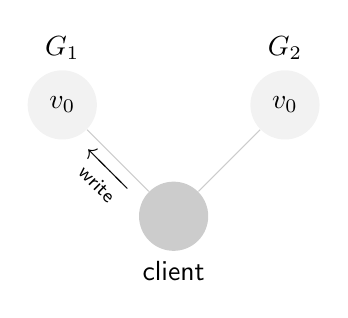
\begin{tikzpicture}[node distance = 2cm]
  \tikzstyle{every state} = [fill=shadecolor, draw=none];
  \tikzstyle{client} = [state, fill=black!20];
  \tikzstyle{clnd} = [-, color=black!20];

  \node[state, label=above:$G_1$] (G1) {$v_0$};
  \node[client, below right of = G1, label=below:client] (cl) {};
  \node[state, above right of = cl, label=above:$G_2$] (G2) {$v_0$};
  
  \draw[clnd] (cl) to node[color=black, sloped, anchor=north, auto=false] 
                      {$\xleftarrow[\textsf{write}]{}$} (G1);
  \draw[clnd] (cl) to (G2);
\end{tikzpicture}
%% node 1 sends 'done' signal to client.
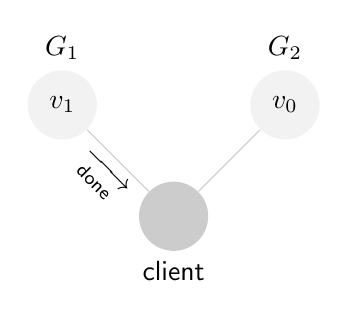
\begin{tikzpicture}[node distance = 2cm]
  \tikzstyle{every state} = [fill=shadecolor, draw=none];
  \tikzstyle{client} = [state, fill=black!20];
  \tikzstyle{clnd} = [-, color=black!20];

  \node[state, label=above:$G_1$] (G1) {$v_1$};
  \node[client, below right of = G1, label=below:client] (cl) {};
  \node[state, above right of = cl, label=above:$G_2$] (G2) {$v_0$};
  \draw[clnd] (cl) to node[color=black, sloped, anchor=north, auto=false] 
                      {$\xrightarrow[\textsf{done}]{}$} (G1);
  \draw[clnd] (cl) to (G2);
\end{tikzpicture}
\end{center}
The consistency demand is now violated, since reading from $G_2$ does not
return the value written by the last completed write operation.
\begin{center}
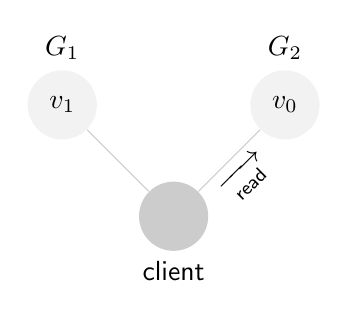
\begin{tikzpicture}[node distance = 2cm]
  \tikzstyle{every state} = [fill=shadecolor, draw=none];
  \tikzstyle{client} = [state, fill=black!20];
  \tikzstyle{clnd} = [-, color=black!20];

  \node[state, label=above:$G_1$] (G1) {$v_1$};
  \node[client, below right of = G1, label=below:client] (cl) {};
  \node[state, above right of = cl, label=above:$G_2$] (G2) {$v_0$};

  \draw[clnd] (cl) to (G1);
  \draw[clnd] (cl) to node[sloped, auto=false, below, text=black] {$\xrightarrow[\textsf{read}]{}$} (G2);

\end{tikzpicture}
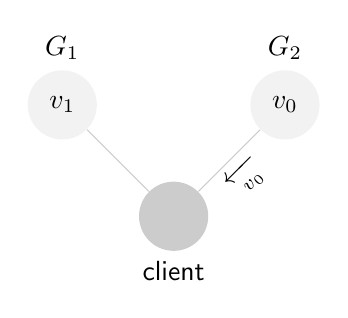
\begin{tikzpicture}[node distance = 2cm]
  \tikzstyle{every state} = [fill=shadecolor, draw=none];
  \tikzstyle{client} = [state, fill=black!20];
  \tikzstyle{clnd} = [-, color=black!20];

  \node[state, label=above:$G_1$] (G1) {$v_1$};
  \node[client, below right of = G1, label=below:client] (cl) {};
  \node[state, above right of = cl, label=above:$G_2$] (G2) {$v_0$};

  \draw[clnd] (cl) to (G1);
  \draw[clnd] (cl) to node[sloped, auto=false, below, text=black] {$\xleftarrow[v_0]{}$} (G2);

\end{tikzpicture}
\end{center}
In conclusion, assuming consistency, availability and partition-tolerance leads
to a contradiction. The above example demonstrates that a partitioned network
can not host a database that is both available and consistent.

\section{Practical consequences of the CAP theorem}
Since the CAP theorem tells us that we can't have partition tolerance while
being consistent and available, this means we need to choose what is most
important for a certain application. Let us discuss a few ways in which
different types of database systems (CA, CP, or AP) can be implemented.



\subsection{Consistent, Available}
A partition-tolerant system can be created by using a single storage
facility. The architecture looks like in Figure~\ref{fig:ca}.
\begin{figure}
\centering
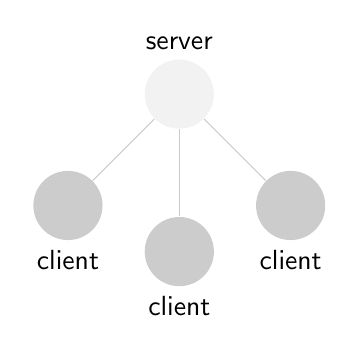
\begin{tikzpicture}[node distance = 2cm]
  \tikzstyle{every state} = [fill=shadecolor, draw=none];
  \tikzstyle{client} = [state, fill=black!20];
  \tikzstyle{clnd} = [-, color=black!20];

  \node[state, label=above:server] (server) {};
  \node[client, below left of = server, label=below:client] (cl1) {};
  \node[client, below  of = server, label=below:client] (cl2) {};
  \node[client, below right of = server, label=below:client] (cl3) {};

  \draw[clnd] (cl1) to (server);
  \draw[clnd] (cl2) to (server);
  \draw[clnd] (cl3) to (server);

\end{tikzpicture}
\caption{Consistent and available: all data on a single node.}
\label{fig:ca}
\end{figure}
There are one or more clients that send requests to a single data storage node.
Requests are handled in order of arrival by the server and a new request is not
handled until the previous one has been completed.  We have consistency since
no synchronisation needs to take place, and since every request to a
non-failing node (a single server node here) will indeed yield a response. The
idea of partition-tolerance becomes irrelevant in this architecture since there
are no data storage nodes to partition by breaking links between them.

The point is that if you want a system that is 100\% Consistent and Available,
you are forced to create a centralized system. Many traditional transactional
database solutions are built this way.

\subsection{Consistent, Partition-tolerant}
Here, we drop availability. The simplest solution for creating a database that
is both consistent and partition tolerant is by building a system where every
node ignores every request. This means that every read operation receives the
same answer: none. It is also partition-tolerant since all nodes always behave
the same and no synchronisation is necessary.

More realistically, a master node can be appointed to distribute data across
nodes, and to queue requests from clients. A read operation cannot take place
before the last write operation is fully complete across all nodes. This means
that when one client issues a request, the others have to wait. An example of
such architecture is shown in Figure~\ref{fig:cp}.
\begin{figure}[h]
\centering
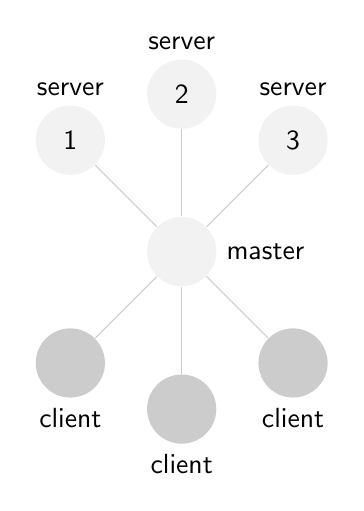
\begin{tikzpicture}[node distance = 2cm]
  \tikzstyle{every state} = [fill=shadecolor, draw=none];
  \tikzstyle{client} = [state, fill=black!20];
  \tikzstyle{clnd} = [-, color=black!20];

  \node[state, label=right:master] (master) {};
  \node[state, above left of = master, label=above:server] (sv1) {1};
  \node[state, above  of = master, label=above:server] (sv2) {2};
  \node[state, above  right of = master, label=above:server] (sv3) {3};
  \node[client, below left of = master, label=below:client] (cl1) {};
  \node[client, below  of = master, label=below:client] (cl2) {};
  \node[client, below right of = master, label=below:client] (cl3) {};

  \draw[clnd] (cl1) to (master);
  \draw[clnd] (cl2) to (master);
  \draw[clnd] (cl3) to (master);
  \draw[clnd] (master) to (sv1);
  \draw[clnd] (master) to (sv2);
  \draw[clnd] (master) to (sv3);


\end{tikzpicture}
\caption{Consistent and partition-tolerant: a single node handles all requests.}
\label{fig:cp}
\end{figure}
Now, if the connection between the master node and server 1 is severed, then
any request that would involve reading from or writing to server 1 will be
dropped (loss of availability). The data that is still reachable on servers 2
and 3 is still consistent across read/write requests.  Such problems can
be avoided by partially duplicating data across servers. An example of this is
Hadoop/HBase. Here, a central node distributes data across multiple nodes.
All data is written to say, three out of $n$ nodes. This means that
availability is only compromised when all three servers that hold a certain
value become unreachable. In practice the probability of such an event may be
low but in terms of the CAP theorem it does mean dropping the Availability
property.

\subsection{Available and Partition-tolerant}
Here we drop the demand that a read request always returns the latest write
result. In Figure~\ref{fig:ap}, a client may write something to one node and
request a value from another node before the write operation has spread across
the network. Or, client 1 may write something to server 1, and client 2 reads
the same information from server 3 before the nodes have synchronized. 
\begin{figure}[h]
\centering
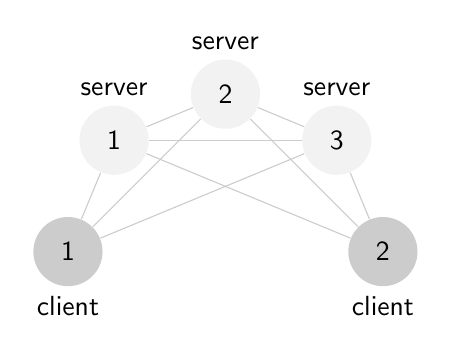
\begin{tikzpicture}[node distance = 2cm]
  \tikzstyle{every state} = [fill=shadecolor, draw=none];
  \tikzstyle{client} = [state, fill=black!20];
  \tikzstyle{clnd} = [-, color=black!20];

  \node[] (center) {};
  \node[client,left of = center, label=below:client] (lclient) {1};
  \node[client,right of = center, label=below:client] (rclient) {2};
  \node[state, above left of = center, label=above:server] (sv1) {1};
  \node[state, above  of = center, label=above:server] (sv2) {2};
  \node[state, above  right of = center, label=above:server] (sv3) {3};

  \draw[clnd] (lclient) to (sv1);
  \draw[clnd] (lclient) to (sv2);
  \draw[clnd] (lclient) to (sv3);
  \draw[clnd] (rclient) to (sv1);
  \draw[clnd] (rclient) to (sv2);
  \draw[clnd] (rclient) to (sv3);
  \draw[clnd] (sv1) to (sv2);
  \draw[clnd] (sv1) to (sv3);
  \draw[clnd] (sv2) to (sv3);

\end{tikzpicture}
\caption{Available and partition-tolerant: there's always a node that answers,
but the servers may not have synchronized information.}
\label{fig:ap}
\end{figure}
An example of such behavior is in social media or online search engines
(Google) where users from different locations may not always get the same
search result at the same time (of course such differences are also obscured by
personalisation).



\section*{Where are we?}
We have seen that there are a few main architectural paradigms on organizing
data in large organizations. These paradigms are based on, and evolve with
practical experience and increasing technological capabilities. The CAP theorem
is a theoretical result that forces one to decide between consistency,
availability or partition-tolerance of a distributed database.


\section{Exercises}
\begin{enumerate}
\item Go to the TOGAF website, and read the
\hlink{https://pubs.opengroup.org/architecture/togaf9-doc/arch/chap01.html\#tag\_01\_03}{Executive
Overview}. Pay attention to how the term `enterprise' is defined.

\item Look up the entries of Data Warehouse, Data Mart, Data Lake,
and Data Virtualisation on Wikipedia. Create a table with pro's and cons
in the columns and an architecture on each row.
\item Using the same system as in Section~\ref{sect:relational:cap},
demonstrate that a distributed database that does not satisfy the availability
condition can be consistent and partition-tolerant. Tips: consider nodes that
can send a `fail' message when they find out that a `write' message is lost.

\item Below are three fictional cases. In this assignment, students are grouped
in teams of 3-5 students. 


Discuss, in about 20-30 minutes, which of the four architectural patterns: Data
Warehouse (DW), Data Mart (DM), Data Lake (DL) or Data Virtualization (DV)
would be preferred. Consider things like the CAP requirements, and realize that
it may be possible to combine strategies. If you have questions about details
in the example just make a reasonable assumption. Feel free to read online
blogs/opinions by data architects for inspiration, or dig up the definitions on
e.g. Wikipedia.


Each team will give a presentation of about 5 minutes, covering the following aspects.
\begin{enumerate}
\item Type of organization as defined in the above description.
\item The choice you made: DW, DM, DL, DV? and
\item most importantly: why you made this choice.
\end{enumerate}
\end{enumerate}


\begin{subappendices}
\section{Cases}
\subsection{The startup}

You work for a fast-growing online startup called `Borkly'. Their product is a
\emph{Next-Generation Search Engine for Old People} with a freemium business model:
customers either use the service for free with adds or choose to take an
add-free subscription with monthly payments. The company works remote-first, so
almost everybody works from home. There are currently 40 people in the company
(not all of them full-time): 3 owner/managers, 22 developers, 5 data analysts
and 10 customer support employees.

For their growing customer support department they are looking to replace their
current ad hoc customer administration (CRM) database backend. The current
system is slow, buggy, and even some simple administrative activities sometimes
take a lot of 'manual' work. There are really only two people who understand how
it works. At the moment Borkly only stores the bare necessities to keep
administration going. In the future they want to be able to store everything
they can get from every customer, including site visits/audit trails, e-mails,
and so on, to be able to serve their data analysts with information.



\subsection{The statistical office}

You work for the \emph{Center of Statistical Information for the Country}. This
bureau is responsible for collecting, producing, and publishing, all national
statistics. It is an organization with about 1000 employees, who all work in the
same building. Although there is one organization, historically each statistical
domain collected and processed its own data, leading to a broad and varying
landscape of data storage solutions, varying from text-files (csv) to
professional data bases. Although such solutions are locally optimal (i.e. they
can be maintained by the departments using them, with some help from the IT
department), management feels that some form of unification would benefit the
Center as a whole.

In the future, the organization would like to cut costs by removing overlapping
information from the organization. They would also like to develop new,
frequently published, statistical products based on the combination of various
data streams in the Center. They would also like data analysts to be able to
quickly create one-off on-demand analysis for external customers. Finally, they
would like to leverage the large quantities of information coming from the
internet of things (IoT) such as mobile phone data for their statistical
products.


\subsection{The government}

You work at the National Office of Employment. This office is responsible for
registering the unemployed, and for payment of unemployment benefits.
Historically, the office was created by merging several regional offices with a
similar task. Although there have been some attempts to unify the legacy data
warehouses into a single data warehouse, the differences between storage
solutions and (meta)data are so large that the office in some respects works
more like a cluster of local offices than as a single unified entity.

The NOE's board recently decided that fraud detection is a spear point within
the organization. To do this it is necessary to integrate both existing data
sources, and new external sources, for example tax records and sometimes social
media records from suspects. The data analyses department is given extra budget
to hire data scientists and they are now talking to the IT department on how to
shape the data landscape.



\end{subappendices}








\chapter{Information modeling}
\label{sect:uml}

In this Chapter we introduce some ideas and methods that have been designed
formally model the entities and relationships that are important for an
organisation. In particular, we will give a brief introduction into Unified
Modeling Language.

\section{Information models} 
An information model is an attempt to capture the essence of the real-life
thing or process in simpler, abstract terms. We have seen an example of an
information model in Chapter~\ref{sect:erd}, when we talked about
Entity-Relationship Diagrams, see also Figure~\ref{fig:erd}.
%
\begin{figure}[h]
\centering
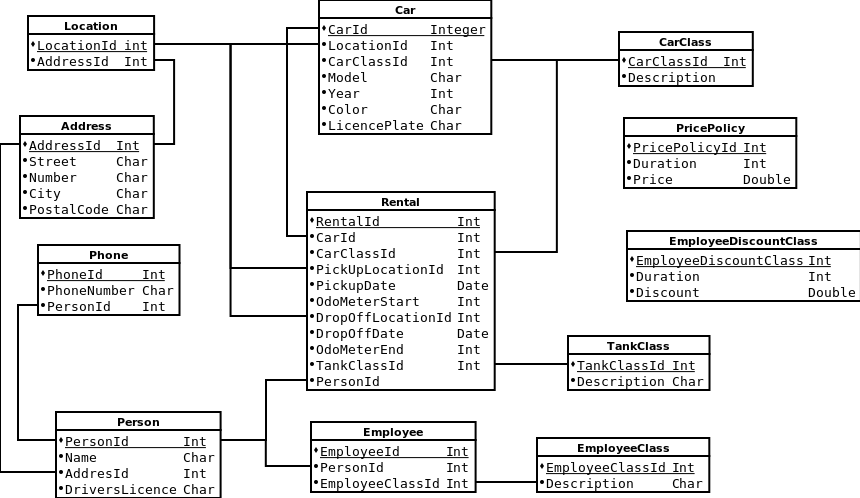
\includegraphics[width=\textwidth]{fig/schema.png}
\caption{An Enterprise-Relationship Diagram}
\label{fig:erd}
\end{figure}

Information models are often separated into three layers, that differ in their
level of detail and precision. The first type is \emph{conceptual}. Conceptual
models are often presented as text or schematic visualisations and their main
purpose is to communicate the bare essentials, for example to high-level
management. There is no formal language for conceptual models, although UML can
be used for this purpose. The second layer is the \emph{logical} information
model (LIM). A LIM describes all information elements in a structured way and
serves as a blueprint for development of for example, a database. A LIM is
typically platform-independent. That is to say, it does not depend on any
particular programming language, database system,  or other implementation
details. Again, UML can be used in this manner but the Entity-Relationship
Diagram of Figure~\ref{fig:erd} is also a good example. The last layer is the
\emph{physical} layer, which describes all technical choices including database
type and configuration input file format, connections to other databases and so
on. 




\section{Introduction to Unified Modeling Language}
UML is a formal graphical language that was developed in the 1990's to cope
with increasing complexity of large software projects. The idea is to
systematically capture all components and the typed relationships between them
in a formal graphical representation that would both be easy to create and easy
to understand. The idea was that ideally, a program can be defined in UML and
the software code can be generated automatically based on the UML
specification. The UML specification itself, is platform-independent and can be
transformed between for example database systems or operating systems.

Like information models in general, UML can be used in roughly three different
ways. It can be used as a sketch tool to outline the most important part of a
process or application. Sketches can be made on a whiteboard or a piece of
paper. Second, it can be used as a blueprinting tool that documents all
components of (for example) a database and the relations between it.  In this
case, it is common to use an UML drawing tool. The resulting document is then
part of the formal specification of a database (or other software system).
Finally, UML can be used as a programming language. Theoretically, if a system
is modeled in enough detail, the UML description can be translated to
executable code on any system where an UML translator  is available. In practice
this is cumbersome and not many applications are developed in that way.

Here we will focus on UML as a sketching tool and treat only a few of the most
important aspects of it. Nevertheless, these aspects can be useful to focus
one's thinking about complex systems or to communicate ideas and designs. Readers
interested in learning more about UML can refer to textbooks, such as that
by \citet{miles2006learning}. 

The main advantages of UML include its generality, understandability and wide
applicability. It can be used to model software, databases, but also the
structure of organisations or physical installations. A disadvantage is that
UML drawings quickly become too large and cluttered to interpret in full. A
more formal disadvantage is that UML is static, in the sense that there is no
algebra of manipulations that allow one to simplify or otherwise manipulate an
UML diagram automatically.

\subsection{Classes and Relations}
UML is used to describe \emph{classes} and their relations.  Term class is an
UML term, and would in the language we've developed in
Chapter~\ref{sect:relational} called an `entity type'. Information objects are
represented as blocks, and relations are represented as possibly decorated
lines between them. The relationships are decorated depending on their type.

The simplest type of relation is an \emph{association}. For example, the
following diagram displays an association between a pet and an owner.
$$

\includegraphics[height=7mm]{fig/pet_owner.png}
$$
Although the box labels are suggestive, in UML this diagram does actually
not say anything about who owns who, or any other property the association
might have. It merely states that a pet is associated with an owner.

\begin{terminology}{Association}
An association between two classes is a relation
that has no direction. It is represented as a solid line between
two information elements.
$$

\includegraphics[height=8mm]{fig/association}
$$
Associations are allowed to have an \emph{arity}, to be labeled, and to have a
direction (See Equation~\ref{eq:labeledassociation}).
\end{terminology}

Classes may be endowed with \emph{attributes} of a certain type. These
properties that may take different values for different elements of the class.
$$
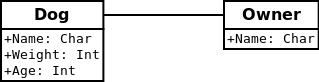
\includegraphics[height=15mm]{fig/pet_owner_attributes.png}
$$
So far, we have done nothing that we have not seen when we discussed
entity-relationship diagrams (Chapter~\ref{sect:erd}). This changes when
we add the \emph{arity} of an association. For example, we can annotate
the association between `Dog' and `Owner' to indicate that a single
Owner is associate with zero or more dogs.
$$
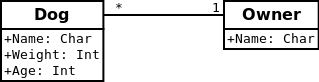
\includegraphics[height=15mm]{fig/pet_owner_arity.png}
$$
Here the asterisk stands for `zero or more' and the 1 stands for, well, one.
%
\begin{terminology}{Arity}
  The \emph{arity} describes the multiplicity on both ends of a relationship.  It
  expresses how many instances of one class can be associated with how many
  instances of another.  The arity is notated at the beginning and end of a
  relation. The notations used are as follows.
  \begin{itemize}
    \item $*$ means 0 or more
    \item $n$, with $n$ a number means `exactly $n$' (for example $n=1$)
    \item $n\ldots m$ means $n,n+1,\ldots,m$.
    \item $n\ldots *$ means $n$ or more.
  \end{itemize}
\end{terminology}

Relations can be labeled, in which case they possibly also gain a direction.
\begin{equation}
\vcenter{\hbox{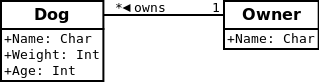
\includegraphics[height=15mm]{fig/pet_owner_labeled_association.png}}}
\label{eq:labeledassociation}
\end{equation}
Here, the owner `owns' a dog. The fact that it is the owner who owns is
signified by the arrow on the label.


Thus far we have discussed associations between classes. A second, more specific
type of relation is the \emph{composition} relation. This occurs when every entity
of a certain class is composed of elements of other classes. Composition is
graphically represented with a solid diamond on the side of the composed class.
$$
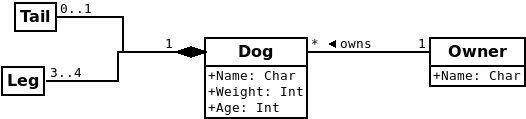
\includegraphics[height=25mm]{fig/pet_owner_composition.png}
$$
Here, a single `Dog' entity is contains 0 or 1 `Tail' entities and 3 to 4 `Leg`
entities. The fact that the lines coming from `Tail' and `Leg` combine before
entering the diamond has no significance; it is just a consequence of the
graphical representation.
\begin{terminology}{Composition}
Composition is an association that describes a part-whole relationship.
The line connecting the two classes is decorated with a solid diamond on the
side of the whole class.
$$

\includegraphics[height=8mm]{fig/composition.png}
$$
\end{terminology}

The last and slightly more complicated type of association we discuss here is
\emph{inheritance}. For any class with a nonempty set of attributes, we can
define a subclass by fixing one or more attributes. For example, we can define
the class `Animal'. If we fix the Boolean attribute `Mammal' to \yay{} and fix
the Species to Dog, we get an inherited class called `Dog'.
$$
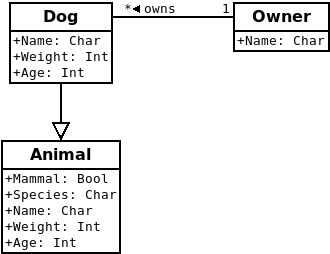
\includegraphics[height=45mm]{fig/pet_owner_inheritance.png}
$$
An equivalent way to think of inheritance is to say that any entity of class
`Dog' is also an `Animal' but not vice versa.

\begin{terminology}{Inheritance}
Inheritance is an association that defines a class-subclass relationship.
It is represented by an arrow, where the arrow points from the subclass to the
superclass.
$$

\includegraphics[height=8mm]{fig/inheritance}
$$
Here `A' is a subclass of `B'. An entity of class `A' has all attributes that
an entity of `B' has, but not the other way around.
\end{terminology}

\subsection{An application in Official Statistics}
\begin{figure}[t]
\centering
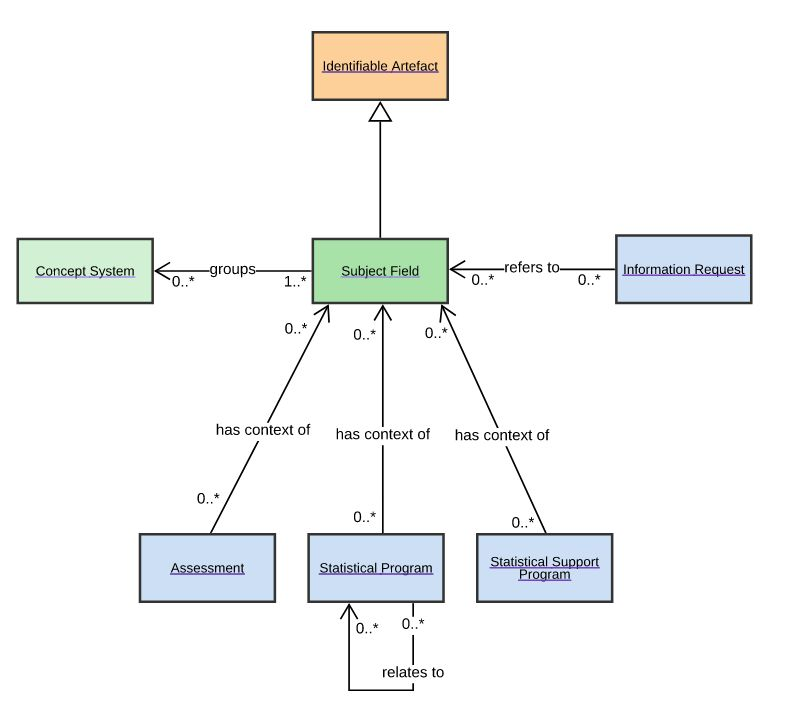
\includegraphics[width=0.7\textwidth]{fig/gsim.jpg}
\caption{The UML diagram surrounding `Subject Field' in the Concept Group of
the General Statistical Information Model. The open arrows indicate the
direction of the label in each association.}
\label{fig:gsim}
\end{figure}
The High-Level Group on Modernisation of Official Statistics (HLG-MOS) is an
initiative of the United Nations Economic Committee for Europe's (UNECE)
Statistical Commission. This initiative is an ongoing effort to both
standardize and modernize how official statistics are produced. HLG-MOS is
steered by a coaliltion of high level managers (typically director general or
deputy director general) who initiate several modernisation projects each year.

In one of these projects, called Generic Statistical Information Model
\hlink{https://statswiki.unece.org/display/gsim/}{(GSIM)}
an attempt was made to model all information objects in a statistical
organisation. The resulting UML diagrams can be found at
\begin{center}
\href{https://statswiki.unece.org/display/gsim/}{\code{https://statswiki.unece.org/display/gsim/}}.
\end{center}
The aim of this effort is not to create databases or software but to have a
reference document that describes the most important things and their
interrelations that are encountered by Official Statistical offices in a
standardized way.  You can think of it as a fancy glossary that can be reused
by statistical organizations. For example by using the same terms for the same
things in their documents and (international) communications. The idea is that
having a common understanding about all these concepts will facilitate common a
understanding of them; having a common understanding again, makes working
together in international context easier.


There are four main UML diagrams covering Business (design and planning of
statistical programs), Concepts (to define the meaning of what data are
measuring), Exchange (to catalogue information entering and exiting an
organization), and Structure (to structure information throughout the
statistical process). Figure~\ref{fig:gsim} shows a piece of the UML diagram
from the `Concepts' group, surrounding the term `Subject Field'. Each such diagram
als comes with a description of the main concept. For example, concept `Subject Field'
comes with the following description.
\begin{center}
\begin{tabular}{|p{0.45\textwidth}|p{0.45\textwidth}|}
\hline
\textbf{Definition} & \textbf{Explanatory text}\\
\hline
One or more \emph{Concept Systems} used for the grouping of \emph{Concepts and
Categories} for the production of statistics.
&
A \emph{Subject Field} is a field of special knowledge under which a set of
\emph{Concepts} and their \emph{Designations} is used. For example, labour
market, environmental expenditure, tourism, etc.\\
\hline
\end{tabular}
\end{center}


%%%%%%%%%%%%%%%%%%%%%%%%%%%%%%%%%%%%%%%%%%%%%%%%%%%%%%%%%%%%%%%%%%%%%%%%%%%%%%%
\section*{Where are we?}
The term `information modeling' refers to a set of techniques that allow one to
systematically describe complex systems. This can be done in ways that vary
from sketchy and high-level to formal and detailed approaches.  The Unified
Modeling Language supports all these approaches and lets the user decide what
level of detail is sufficient for their purpose.

\section{Exercises}
\label{sect:exinfomodel}

\begin{enumerate}
\item Describe the classes and relationships between them for each of the
following UML diagrams.
\begin{enumerate}
\item
$$
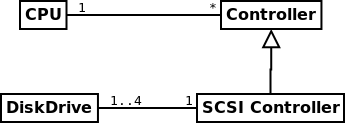
\includegraphics[height=25mm]{fig/ex_2_computer.png}
$$
\item
$$
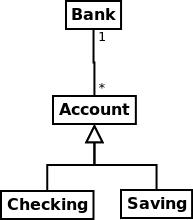
\includegraphics[height=45mm]{fig/ex_3_bank.png}
$$
\end{enumerate}
\item Complete the UML diagram of Figure~\ref{fig:erd}, see also Case~\ref{sect:schema} for a
full description. You can draw your own diagram or use the diagram on page~\pageref{pg:diagram}.
\end{enumerate}
\hfill{}Check your answers on page~\pageref{sect:ansinfomodel}.

\newpage
\begin{figure}[!h]
\centering
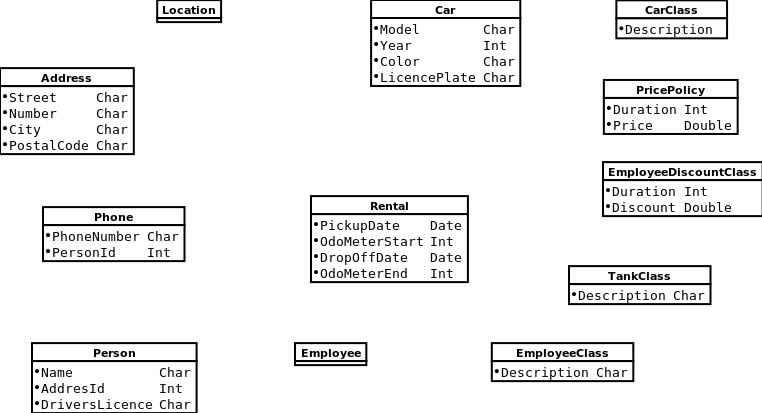
\includegraphics[height=0.8\textwidth,angle=90]{fig/uml_exercise.png}
\end{figure}
\label{pg:diagram}






\addcontentsline{toc}{chapter}{Bibliography}
\bibliography{datamanagement}

\appendix
\chapter{Answers to selected exercises}
\label{sect:answers}

%%%%%%%%%%%%%%%%%%%%%%%%%%%%%%%%%%%%%%%%%%%%%%%%%%%%%%%%%%%%%%%%%%%%%%%%%%%%%%%
\section*{Answers for section \ref{sect:exfaces}}
\label{sect:ansfaces}
\begin{enumerate}
  \item For data that is stored (in a database) and data that is transported
        we want each value to be described unambiguously. Here, we have
        two values where `fuel' is described as `-- of which bio'. This makes
        interpretation dependent on the order of records.
  \addtocounter{enumi}{2}
\item 
  \begin{enumerate}
  \item Not suited.%: the entities are in columns and their properties in rows.
  \item Not suited.%: the column names are values of a `hidden' property: income class.
  \item Suited for analyses (but note that a 5-year old has a job in this data,
        so the data is invalid).
  \item Not suited.% the last row is not en entity from the population of `types of businesses`.
        %(Think of the rule of thumb: is the sum over the `costs' column a meaningful number?).
  \end{enumerate}
  \item Basically anything that you can do with image-processing software, e.g.: format conversion
        from png to jpg, zoom, blur, rotate, flip, and so on. A counter example is Optical Character
        Recognition, where image data is converted to character strings.
  \item \begin{enumerate}
  \item True. %for any two natural numbers $a$ and $b$, $a\cdot b$ is also a natural number.
  \item True. %obviously. But let's prove it. Any member of $\mathbb{Q}$ can be written 
        %in the form $\frac{p}{q}$, where $p$ and $q$ are in $\mathbb{N}$. Now consider the
        %addition $x = \frac{a}{b}+\frac{c}{d}$. Multiplying each term with 1 (written as $d/d$ or
        %$b/b$,  we can write $x = \frac{ad}{db}+\frac{cb}{db}=\frac{ad+cb}{db}$, which is indeed
        %of the form $\frac{p}{q}$ (because $\mathbb{N}$ is closed under addition and multiplication).
  \item False. %because for example both 1 and 0 are real numbers, but $1/0$ is not.
  \item True. %since $\textsf{zero}(n)=0$ for any $n\in\mathbb{Z}$ and $0\in\mathbb{Z}$.
  \item False. %Since $\textsf{4}=0$ and $0\not\in\mathbb{N}$.
  \item False. %Although there are an infinite number of integers, infinity itself is not
        %a number in $\mathbb{N}$.
  \end{enumerate}
\end{enumerate}


%%%%%%%%%%%%%%%%%%%%%%%%%%%%%%%%%%%%%%%%%%%%%%%%%%%%%%%%%%%%%%%%%%%%%%%%%%%%%%%
\section*{Answers for section \ref{sect:exsvc}}
\label{sect:anssvc}
\begin{enumerate}
\item
  \begin{enumerate}
  \item Between raw and input, or between statistics and output.
  \item Between valid and statistics, or perhaps between input and valid as auxiliary information.
  \item Between raw and input.
  \item Between raw and input.
  \item Between raw and input.
  \end{enumerate}
\end{enumerate}


%%%%%%%%%%%%%%%%%%%%%%%%%%%%%%%%%%%%%%%%%%%%%%%%%%%%%%%%%%%%%%%%%%%%%%%%%%%%%%%
\section*{Answers for section \ref{sect:exvalidation}}
\label{sect:ansvalidation}
\begin{enumerate}
  \item
  \begin{enumerate}
    \item $D = \{\texttt{yes}, \texttt{no}, \texttt{under-aged}, \texttt{adult},\texttt{retired}\}$.
    \item $K = \{(Alice, Job), (Alice, Age), (Bob, Job), (Bob, Age)\}$.
    \item Four keys, and for each we have 5 options, so the size of $D^K$ equals $5^4=625$.
  \end{enumerate}
  \item There are 4 valid job-age combinations, and 2 persons, so $4^2=16$ possibilities.
  \item
  \begin{enumerate}
    \item validation rule.
    \item not a validation rule.
    \item not a validation rule.
  \end{enumerate}
  \item
  \begin{enumerate}
    \item $smms$, validation level 2.
    \item $ssms$, validation level 1.
    \item $ssms$, validation level 1.
    \item $mmmm$, validation level 4.
    \addtocounter{enumi}{1}
  \end{enumerate}
  \item \verb+total_rev >= 0+
  \item $age \geq 0$, $income \geq 0$
  \item \verb+income <= 0+
  \item \verb+age >= 12+ can be left out.
\end{enumerate}


%%%%%%%%%%%%%%%%%%%%%%%%%%%%%%%%%%%%%%%%%%%%%%%%%%%%%%%%%%%%%%%%%%%%%%%%%%%%%%%
\section*{Answers for section \ref{sect:exrelational}}
\label{sect:ansrelational}

\begin{enumerate}
\item
  \begin{tabular}{|cccc|}
  \hline
  Id & Name  & Age & Owns \\
  \hline
  1  & Alice & 7 & $\{\textrm{puzzle}\}$\\
  1  & Alice & 7 & $\{\textrm{bicycle}\}$\\
  2  & Bob   & 6 & $\{\textrm{ball}\}$\\
  \hline
  \end{tabular}

\item 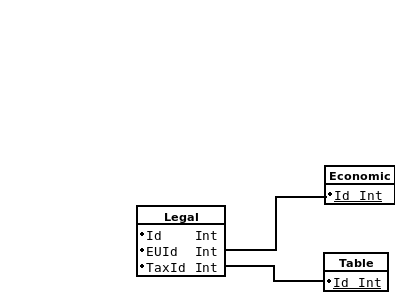
\includegraphics[height=45mm]{fig/units.png}

\item
  \begin{enumerate}
    \item 15 (including the primary and foreign keys).
    \item AlbumId, MediatypeId, GenreId.
    \item Integer
  \end{enumerate}

\item See figure~\ref{fig:ansschema} on page \pageref{fig:ansschema}.
  \begin{figure}[p]
  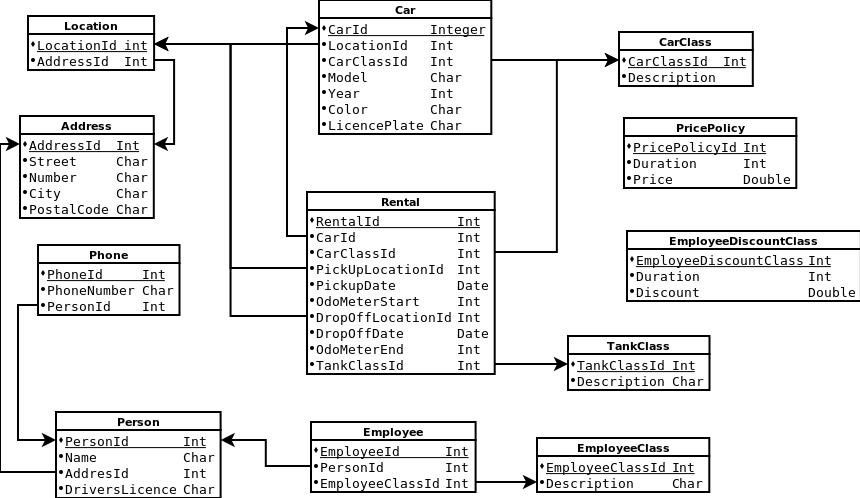
\includegraphics[width=\textwidth]{fig/schema_rentals.png}
  \caption{Car rental ERD.}
  \label{fig:ansschema}
  \end{figure}

\item $\{a,b,c,d,e\}\cap\{b,d,f\}=\{b,d\}$. Furthermore $V\cup W = \{a,b,c,d,e,f\}$,
      $V-W=\{a,c,e\}$, and $W-V=\{f\}$. So $\{a,b,c,d,e,f\}-\{a,c,e\}-\{f\}=\{b,d\}$.
\item 
  \begin{enumerate}
  \item $\Pi_{a\in A}(A\ltimes B) = A$ (note: this is true for any $A$).

  \item 
  $
  \sigma_{Age>40} (A\times B) = \sigma_{Age>40}(A)\times B
  =
  \begin{array}{|lll|}
  \hline
  Name & Age & Height\\
  \hline
  \hline
  \end{array}
  $ (table with zero rows and three columns).
  \item 
  \begin{align*}
  \sigma_{Age\leq40\land Height\leq 170} (A\times B) &= 
    \sigma_{Age\leq 40}(A)\times\sigma_{height\leq 170}(B)\\
  & =
  \begin{array}{|lll|}
  \hline
  Name & Age & Height\\
  \hline
  Mary & 34  & 167\\
  \hline
  \end{array}
  \end{align*}

  \item
  $$
  \Pi_{Height}A\bowtie B 
  = 
  \begin{array}{|l|}
  \hline
   Height\\
  \hline
   178\\
   167\\
  \hline
  \end{array}
  $$
  \end{enumerate}

\item
\begin{enumerate}
\item $\Pi_{Title,Name}(\texttt{tracks}\ltimes_{AlbumId}\texttt{albums})$
\item For readability we define two intermediate results: $X$ and $Y$.
\begin{align*}
X & = \texttt{tracks}\ltimes_{AlbumId}(\texttt{albums}\ltimes_{ArtistId}(\rho_{Name/Artist}\texttt{artists}))\\
Y & = (\texttt{invoice\_items}\ltimes_{TrackId}X)\bowtie\texttt{invoices}\bowtie_{CustomerId}\texttt{customers}\\
& \Pi_{Artist,Name,CustomerId}(Y)
\end{align*}
\item $\Pi_{TrackId,EmployeeId}(Y\bowtie\texttt{employees})$.
\end{enumerate}
\end{enumerate}


%%%%%%%%%%%%%%%%%%%%%%%%%%%%%%%%%%%%%%%%%%%%%%%%%%%%%%%%%%%%%%%%%%%%%%%%%%%%%%%
\section*{Answers for section \ref{sect:exinfomodel}}
\label{sect:ansinfomodel}

\begin{enumerate}
\item
  \begin{enumerate}
  \item One CPU is associated with 0 or more controllers. An SCSI Controller
        is a type of controller. One SCSI controller is associated with 1 to 4
        DiskDrives.
  \item One Bank is associated with 0 or more Accounts. Checking and Saving
        are types of Accounts.
  \end{enumerate}
  \item  See Figure~\ref{fig:ansuml} on page \pageref{fig:ansuml}.
  \begin{figure}[p]
  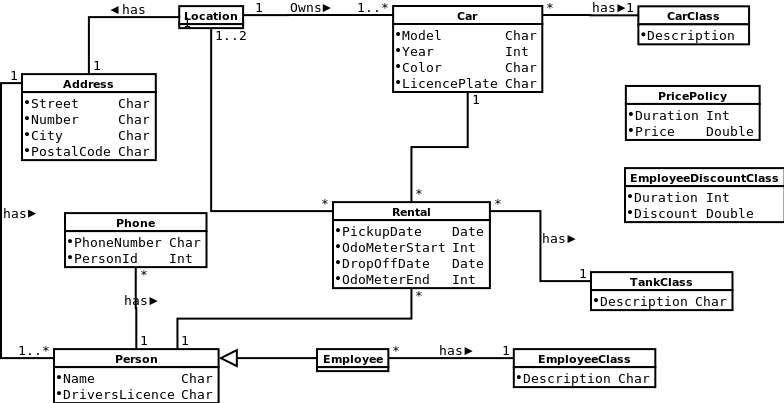
\includegraphics[width=\textwidth]{fig/umldiagram.png}
  \caption{Car rental UML diagram.}
  \label{fig:ansuml}
  \end{figure}
\end{enumerate}




\addcontentsline{toc}{chapter}{Index}
\printindex


\end{document}

